%% 
%% Copyright 2007-2020 Elsevier Ltd
%% 
%% This file is part of the 'Elsarticle Bundle'.
%% ---------------------------------------------
%% 
%% It may be distributed under the conditions of the LaTeX Project Public
%% License, either version 1.2 of this license or (at your option) any
%% later version.  The latest version of this license is in
%%    http://www.latex-project.org/lppl.txt
%% and version 1.2 or later is part of all distributions of LaTeX
%% version 1999/12/01 or later.
%% 
%% The list of all files belonging to the 'Elsarticle Bundle' is
%% given in the file `manifest.txt'.
%% 

%% Template article for Elsevier's document class `elsarticle'
%% with numbered style bibliographic references
%% SP 2008/03/01
%%
%% 
%%
%% $Id: elsarticle-template-num.tex 190 2020-11-23 11:12:32Z rishi $
%%
%%
\documentclass[preprint,5p,twocolumn]{elsarticle}

\usepackage{amsmath,amssymb,amsfonts,amsthm}
\usepackage{algorithmic}
\usepackage{graphicx}
\usepackage{textcomp}
\usepackage{xcolor}
\usepackage{pifont}
\usepackage{tikz}
\newtheorem{theorem}{Theorem}
\newtheorem{lemma}[theorem]{Lemma}
\newtheorem{definition}[theorem]{Definition}
\newtheorem{problem}[theorem]{Problem}
\newtheorem{remark}[theorem]{Remark}
\newtheorem{corollary}[theorem]{Corollary}
\newtheorem{proposition}[theorem]{Proposition}

%% Use the option review to obtain double line spacing
%% \documentclass[authoryear,preprint,review,12pt]{elsarticle}

%% Use the options 1p,twocolumn; 3p; 3p,twocolumn; 5p; or 5p,twocolumn
%% for a journal layout:
%% \documentclass[final,1p,times]{elsarticle}
%% \documentclass[final,1p,times,twocolumn]{elsarticle}
%% \documentclass[final,3p,times]{elsarticle}
%% \documentclass[final,3p,times,twocolumn]{elsarticle}
%% \documentclass[final,5p,times]{elsarticle}
%% \documentclass[final,5p,times,twocolumn]{elsarticle}

%% For including figures, graphicx.sty has been loaded in
%% elsarticle.cls. If you prefer to use the old commands
%% please give \usepackage{epsfig}

%% The amssymb package provides various useful mathematical symbols
\usepackage{amssymb}

%% The amsthm package provides extended theorem environments
%% \usepackage{amsthm}

%% The lineno packages adds line numbers. Start line numbering with
%% \begin{linenumbers}, end it with \end{linenumbers}. Or switch it on
%% for the whole article with \linenumbers.
%% \usepackage{lineno}

\journal{Information Processing Letters}

\begin{document}

\begin{frontmatter}

%% Title, authors and addresses

%% use the tnoteref command within \title for footnotes;
%% use the tnotetext command for theassociated footnote;
%% use the fnref command within \author or \address for footnotes;
%% use the fntext command for theassociated footnote;
%% use the corref command within \author for corresponding author footnotes;
%% use the cortext command for theassociated footnote;
%% use the ead command for the email address,
%% and the form \ead[url] for the home page:
%% \title{Title\tnoteref{label1}}
%% \tnotetext[label1]{}
%% \author{Name\corref{cor1}\fnref{label2}}
%% \ead{email address}
%% \ead[url]{home page}
%% \fntext[label2]{}
%% \cortext[cor1]{}
%% \affiliation{organization={},
%%             addressline={},
%%             city={},
%%             postcode={},
%%             state={},
%%             country={}}
%% \fntext[label3]{}

\title{Interactive Noninterference Does Not (Always) Compose}

%% use optional labels to link authors explicitly to addresses:
%% \author[label1,label2]{}
%% \affiliation[label1]{organization={},
%%             addressline={},
%%             city={},
%%             postcode={},
%%             state={},
%%             country={}}
%%
%% \affiliation[label2]{organization={},
%%             addressline={},
%%             city={},
%%             postcode={},
%%             state={},
%%             country={}}

\author[inst1]{François Hublet}

\affiliation[inst1]{organization={ETH Zürich},%Department and Organization
            addressline={CNB F 107.2, Universitätstrasse 6},
            city={Zürich},
            postcode={8051},
            country={Switzerland}}
\begin{abstract}
  We study the notion of Interactive Noninterference (INI) as introduced by
  O'Neill et al.~\cite{ONeill2006} and Rafnsson et al.~\cite{Rafnsson2012}.
  We show that, unlike claimed in previous work, INI is generally not compositional when
  programs are non-deterministic. To this end, we exhibit elementary attacks on INI that cover
  both blocking and non-blocking communication between interactive programs. Then, we
  prove that compositionality can be recovered in at least four ways:
  by requiring programs to be deterministic,
  by using a total-order lattice or public presence labels, or by fulfilling a stronger \emph{coalition INI} (CINI)
  property. All definitions and results of this paper have been formally verified in the Lean 4 proof assistant.
\end{abstract}

%%Graphical abstract
%\begin{graphicalabstract}
%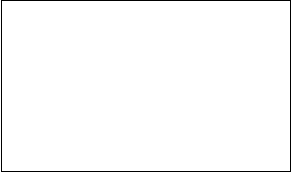
\includegraphics{grabs}
%\end{graphicalabstract}

%%Research highlights
%\begin{highlights}
%\item Research highlight 1
%\item Research highlight 2
%\end{highlights}

\begin{keyword}
%% keywords here, in the form: keyword \sep keyword
non-interference \sep interactive programs \sep compositionality
%% PACS codes here, in the form: \PACS code \sep code
%\PACS 0000 \sep 1111
%% MSC codes here, in the form: \MSC code \sep code
%% or \MSC[2008] code \sep code (2000 is the default)
%\MSC 0000 \sep 1111
\end{keyword}

\end{frontmatter}

%% \linenumbers

%% main text
\newcommand{\xmark}{{\color{red}\ding{55}}}%
%\definecolor{darkgreen}{rgb}{0.13, 0.55, 0.13}
\newcommand{\cmark}{{\color{darkgreen}\checkmark}}%


\newcommand{\sA}{s_{\mathtt{A}}}
\newcommand{\sB}{s_{\mathtt{B}}}
\newcommand{\sC}{s_{\mathtt{C}}}
\newcommand{\sD}{s_{\mathtt{D}}}
\newcommand{\sE}{s_{\mathtt{E}}}
\newcommand{\sF}{s_{\mathtt{F}}}
\newcommand{\PA}{P_{\mathtt{A}}}
\newcommand{\PB}{P_{\mathtt{B}}}
\newcommand{\PC}{P_{\mathtt{C}}}
\newcommand{\pOut}[2]{\mathtt{out}_{#1}(#2)}
\newcommand{\pIn}[2]{\mathtt{in}_{#1}(#2)}
\newcommand{\pAssign}[2]{#1 := #2}
\newcommand{\pComp}[2]{#1 \mid #2}
\newcommand{\Lattice}{\mathcal{L}}
\renewcommand{\doteq}{\overset{.}{=}}
\newcommand{\Pow}[1]{\mathcal{P}(#1)}
%% Pointer to the accompanying Lean 4 development.
\newcommand{\leanref}[1]{\hfill\textnormal{\small\textsf{[Lean:\,\texttt{#1}]}}}


% TODO: Randomness vs. Nondeterminism
\section{Introduction}

\emph{Interactive programs} were introduced by O'Neill, Clarkson, and Chong~\cite{ONeill2006} as a model
for imperative programs that interact with users through inputs and outputs while updating
their state. In interactive programs, users can adapt their outputs depending on previously
seen inputs in a malicious way, which provides additional avenues for information leakage.
To illustrate these challenges, O'Neill et al.~\cite{ONeill2006} use the following
example, where $\mid$ denotes non-deterministic choice and $\oplus$ stands for `exclusive or':
\begin{align*}
  P_0=~&(\pComp{\pAssign{x}{0}}{\pAssign{x}{1}}); \pOut{H}{x}; \pIn{H}{y}; \pOut{L}{x \oplus y}.
\end{align*}
At first glance, program $P_0$ does not seem to propagate information from high to low channels, as
the high information input from channel $H$ is \emph{xor}ed with the random value in $x$ before being
output to $L$. However, attacks become possible when interaction is considered. Suppose that Hillary,
who can read and write on channel $H$, wants to send a bit of information $b$ to Laura, who can read only
on channel $L$. Hillary can simply observe the bit $x$ and set $y$ to $b \oplus x$; then Laura will read
$x \oplus y = x \oplus (b \oplus x) = b$ on $L$, which is exactly the bit Hillary wanted to transmit.

To guarantee that no information flows from high to low channels in interactive programs, the notion
of interactive noninterference~\cite{ONeill2006} (INI) has been introduced. INI relies on \emph{strategies}
that encode how users with different clearance levels provide new inputs depending on the outputs
they have been able to observe up to the present. In the above example, INI is violated because
there exist two strategies differing only on the high channel (the one where Hillary transmits $1$ and the one she transmits $0$) that produce different outputs on the low channel.

This initial study on interactive programs gave rise to a number of follow-up works.
Clark and Hunt~\cite{Clark2008} showed that, in the case of \emph{deterministic} interactive
programs, considering general strategies was not needed. They showed that those programs satisfying INI
were exactly those satisfying noninterference for \emph{stream strategies} where the sequence of user
inputs is fixed ahead of time independently of any outputs. Later, Rafnsson, Hedin, and Sabelfeld
reconsidered the general case~\cite{Rafnsson2012}, revisiting it in two different directions. First, they
extended O'Neill et al.'s model to support \emph{non-total} strategies in which channels may not always
contain data ready to be input, and for which the \emph{presence} and \emph{value} of data on a given channel
may have different security levels. In their model, a channel has levels, e.g., $H^L$, if the
presence of an input on it is public, but the value of the input is private.
Second, Rafnsson et al. studied the compositionality of INI. They claimed that INI on their two-level model
was compositional for both deterministic and non-deterministic programs, and provided a type system to statically
check for INI in imperative programs.

For interactive non-interference to be useful in real-world software systems, compositionality is arguably
a key property. Indeed, most privacy-sensitive systems that interact with users
are component-based, e.g., because they are multi-tier or run on a microservice architecture.
In general, being able to check for non-interference component-wise rather than globally results
in a significant reduction in the complexity of the verification process.
Even more critically, it might be the only practical approach when dealing with systems that
combine components from multiple code providers that may not be willing to share their sources.

Unfortunately, and as we will show in the first part of this paper, the compositionality property claimed
by Rafnsson et al. for INI~\cite[Theorem V.1]{Rafnsson2012} does not hold. Elementary attacks against
INI exist for non-deterministic programs in both Rafnsson et al.'s non-total (blocking) setup and the original
total (non-blocking) setup by O'Neill et al.~\cite{ONeill2006}, who did not make any compositionality claims.
The compositionality proofs provided in the original paper~\cite{Rafnsson2012} contains an error. In the second part of this paper,
we show that compositionality can be recovered in four ways:
(a) by considering only \emph{deterministic programs},
for which Rafnsson et al.'s result holds;
(b) by considering only lattices that are \emph{total orders};
(c) by making all presence labels public; or
(d) by strengthening INI to a stronger \emph{coalition INI} (CINI) and imposing
an additional restriction on presence labels.

After reviewing interactive noninterference as introduced by O'Neill et al. and Rafnsson et al.~\cite{ONeill2006,Rafnsson2012}
(Section~\ref{sec:preliminaries}), we make the following contributions:
\begin{itemize}
\item We show that INI is non-compositional in both total and non-total setups by exhibiting elementary
  attacks. We also briefly review the flawed proof presented in previous work and identify the mistake it contains.
  (Section~\ref{sec:non-compositionality})
\item We show that INI is compositional when all programs are deterministic (Section~\ref{sec:deterministic}).
\item We propose \emph{coalition INI} (CINI), a natural strengthening of
  INI in which observers pool
  their knowledge (Definition~\ref{def:coalition}), and show that it is compositional
  under an additional condition on presence labels.
  Coalition-noninterference does not compose when this condition is dropped.
  As a corollary, we obtain compositionality of INI for total orders and with public presence labels
  (Section~\ref{sec:coalition composes}).
\item We formalize the entire development in the Lean 4 proof assistant, and machine-check all of its
  proofs.\footnote{The accompanying development consists of the file \texttt{InteractiveNI.lean} and
  the directory \texttt{InteractiveNI/}. It uses no external dependencies and contains
  no \emph{sorries}. Each definition, lemma and
  theorem below is annotated with the name of its Lean counterpart.}
\end{itemize}

\subsection{Related work}

Compositionality has been a central concern of information-flow security since the 
introduction of seminal definitions of nondeducibility~\cite{Sutherland1986} and 
noninterference~\cite{Goguen1984} for input-output systems in the mid-1980s.
Shortly thereafter, McCullough observed that these definitions do not
compose~\cite{McCullough1988}, and proposed \emph{restrictiveness}
as a stronger, compositional property under nondeterminism~\cite{McCullough1990}.
Zakinthinos and Lee later showed that composability of standard noninterference could be
recovered by removing or delaying feedback loops between components~\cite{Zakinthinos1995},
characterized its failure modes~\cite{Zakinthinos1996},
and proved that the minimal properties ensuring noninterference do compose~\cite{Zakinthinos1997}.
Mantel later systematized previous work on the composability of security properties of
input-output systems~\cite{Mantel2002} and extended his framework to support assumptions
and guarantees on inputs and outputs~\cite{Mantel2011}. These early works provided the
base for many developments in language-based noninterference, in which compositionality
is a key requirement~\cite{Sabelfeld2000,Mantel2003,Karbyshev2018,Frumin2021}.

The setting adopted in this paper---programs interacting with users \emph{during} execution---was
introduced by O'Neill et al.~\cite{ONeill2006}, building on the strategies of Wittbold and
Johnson~\cite{Wittbold1990}. Early on, Millen had shown that nondeducibility on strategies
was compositional for a restricted class of \emph{synchronized machines}~\cite{Millen1990}.
In O'Neill's setup, Clark and Hunt~\cite{Clark2008} proved compositionality for deterministic programs.
Rafnsson et al.~\cite{Rafnsson2012,Rafnsson2014} extended O'Neill et al.'s model
with non-total strategies and separate presence and value levels, and stated the
compositionality result that we are set to disprove.
Compositionality on stream semantics was further developed by Rafnsson and
Sabelfeld~\cite{RafnssonSabelfeld2014} in a significantly different setup---we do not examine their
results here, nor do we claim that our results affect their other conclusions in any way.

Formal verification of noninterference is standard (see, e.g.~\cite{Popescu2013}).

\section{Interactive Noninterference}

\label{sec:preliminaries}

\newcommand{\Strat}{\mathbf{Strat}}
\newcommand{\StratT}{\mathbf{Strat}_{\mathrm{T}}}
\newcommand{\StratNI}{\mathbf{Strat}\text{-}\mathrm{NI}}
\newcommand{\StratTNI}{\mathbf{Strat}_{\mathrm{T}}\text{-}\mathrm{NI}}
\newcommand{\States}{\mathbb{S}}
\newcommand{\IO}{\mathrm{IO}}
\newcommand{\Channels}{\mathbb{C}}
\newcommand{\Values}{\mathbb{V}}
\newcommand{\Traces}{\mathbb{T}}

In this section, we recall the definitions of interactive programs, strategies, and interactive non-interference (INI) as presented by Rafnsson et al.~\cite{Rafnsson2012}. %All notions introduced below are formalized in \texttt{InteractiveNI/Basic.lean}, respectively as \texttt{Sec} (security context), \texttt{Reach} ($\xrightarrow{t}$), \texttt{Deterministic}, \texttt{parStep} and \texttt{parStepFam} (composition), \texttt{proj} and \texttt{teq} ($\pi_\ell$ and $=_\ell$), \texttt{Strategy}, \texttt{seq} ($=_\ell$ on strategies), \texttt{consistent}, \texttt{produces} ($\vDash$), and \texttt{INI}.

\subsection{Interactive programs}

In the following, we fix a set $\Channels$ of channel symbols and a set $\Values$ of values.
Variables $\alpha, \alpha', \dots$ denote channels and $v, v', \dots$ denote values.
Each channel $\alpha$ is mapped to a pair of security levels $(\ell_2,\ell_1)$ taken from a
semilattice $(\Lattice, \sqsubseteq)$ through a mapping $\gamma : \Channels \rightarrow \Lattice^2$. This pair is also denoted $\ell_1^{\ell_2}$. The superscripted level $\ell_2$ captures
the confidentiality of the \emph{presence} of a message on $\alpha$, while level 
$\ell_1$ captures the confidentiality of the \emph{values} of messages on $\alpha$.
Since the value of a message cannot be observed without observing its presence, we require
$\ell_2 \sqsubseteq \ell_1$ throughout.

We fix a set $\IO$ of \emph{input-output labels} containing all labels of the form
$\alpha ? v$ (denoting input of $v$ on $\alpha$), $\alpha ! v$ (denoting output of $v$ to $\alpha$), or $\tau$ (denoting no input or output).
We write $\alpha : v$ for a label that is either $\alpha ? v$ or $\alpha ! v$; within a single
formula, all occurrences of `$:$' denote the same direction.
Using this set, our model of interactive programs, called
\emph{input-output labeled transition systems} or IOLTS~\cite{Rafnsson2012}, is defined as follows:

  \label{def:iolts}
\begin{definition}
  An \emph{input-output labeled transition system} (IOLTS) is a pair $(\States, \rightarrow)$ such that:
  \begin{enumerate}[(i)]
  \item $\States$ is a set of states,
  \item $\rightarrow \subseteq \States \times \IO \times \States$ is a transition system,
  \item $(\States, \rightarrow)$ is \emph{input-neutral}, i.e.,
  \begin{align*}
    \forall s, s' \in \States, \alpha \in \Channels, v \in \Values.\\
    s \xrightarrow{\alpha ? v} s' \Longrightarrow (\forall v' \in \Values.\,\exists s'' \in \States.\,s \xrightarrow{\alpha ? v'} s'')
  \end{align*}
  \end{enumerate}
\end{definition}

An IOLTS is thus a labelled transition system whose labels are split into
inputs, outputs and a silent action, with the additional requirement that a state ready to
read on a channel be ready to read \emph{any} value on it. %Readers familiar with automata theory
%may find it helpful to think of the deterministic case as a Mealy machine whose input alphabet is
%$\Channels \times \Values$, the difference being that inputs are supplied by the strategies of
%Section~\ref{sec:strategies} rather than by a fixed input word.

The setup considered by O'Neill et al.~\cite{ONeill2006} is similar but has only one level
per channel, corresponding to the value level above. As a result, the presence of messages on a
channel is always considered public. This is consistent with the authors' assumption that
all channels can be read from at all times.

An IOLTS is considered deterministic when in any state, the next state only depends on the
current state and, possibly, on a single input on a fixed channel.

\begin{definition}
  \label{def:deterministic}
  An IOLTS $(\States, \rightarrow)$ is deterministic iff, for all $s,s',s'' \in \States$ and
  $a,a' \in \IO$ such that $s \xrightarrow{a} s'$ and $s \xrightarrow{a'} s''$:
  \begin{enumerate}[(i)]
  \item if $a \neq a'$, then $a = \alpha ? v$ and $a' = \alpha ? v'$ for some $\alpha,v,v'$; and
  \item if $a = a'$, then $s' = s''$.
  \end{enumerate}
\end{definition}

\emph{Executions} $s \xrightarrow{t} s'$, where the word $t$ is the \emph{trace} they generate,
are defined inductively: $s \xrightarrow{\varepsilon} s$ for all $s \in \States$, where
$\varepsilon$ is the empty trace; if $s \xrightarrow{\tau} s'$ and $s' \xrightarrow{t} s''$, then
$s \xrightarrow{t} s''$; and if $s \xrightarrow{\alpha : v} s'$ and $s' \xrightarrow{t} s''$, then
$s \xrightarrow{\alpha : v . t} s''$. Silent steps thus leave no mark on the trace.
The set of traces is denoted by $\Traces$.
In the following, variables $t, t', t_1, t_2, \dots$ implicitly range over $\Traces$.

Two traces are called \emph{equivalent} with respect to a level $\ell \in \Lattice$
(`$\ell$-equivalent') when they differ only by the presence of inputs or outputs on channels with
a presence level $\ell_2 \not\sqsubseteq \ell$, and by the value of inputs or outputs on channels
with a value level $\ell_1 \not\sqsubseteq \ell$. Intuitively, an agent that is only able to
observe the presence of inputs or outputs on channels with presence level $\sqsubseteq \ell$ and the value of
inputs or outputs on channels with value level $\sqsubseteq \ell$ should not be able to distinguish the two
traces. Formally:
\begin{definition}
  \label{def:projection}
  For any $\ell \in \Lattice$, two traces $t,t'$ are $\ell$-equivalent, denoted $t =_\ell t'$, iff
  $\pi_\ell(t) = \pi_\ell(t')$, where $\pi_\ell$ is defined inductively as follows:
  \begin{align*}
    \pi_\ell(\varepsilon) &=  \varepsilon \\
    \pi_\ell(\alpha : v.t) &= \pi_\ell(t) & & \text{if } \gamma(\alpha)=\ell_1^{\ell_2}, \ell_2 \not\sqsubseteq \ell\\
    \pi_\ell(\alpha : v.t) &= \alpha : \square. \pi_\ell(t) & & \text{if } \gamma(\alpha)=\ell_1^{\ell_2}, \ell_1 \not\sqsubseteq \ell, \ell_2 \sqsubseteq \ell\\
    \pi_\ell(\alpha : v.t) &= \alpha : v . \pi_\ell(t) & & \text{if } \gamma(\alpha)=\ell_1^{\ell_2}, \ell_1\sqsubseteq \ell,\ell_2 \sqsubseteq \ell,
  \end{align*}
  where $: \in \{?,!\}$.
\end{definition}

%Since $\pi_\ell(t.t') = \pi_\ell(t).\pi_\ell(t')$, the relation $=_\ell$ is a congruence for
%concatenation: $t_1 =_\ell t'_1$ and $t_2 =_\ell t'_2$ imply $t_1.t_2 =_\ell t'_1.t'_2$. We use
%this fact repeatedly and without further mention.

Composition of a family of IOLTS is defined naturally as arbitrary interleaving of component-wise
steps on the product of the IOLTS's states.

\begin{definition}
  Let $I$ be a set of indices. The \emph{parallel composition} (short \emph{composition}) of a family of IOLTS $(\States_i,\rightarrow_i)_{i \in I}$ is the IOLTS $(\bigotimes_{i \in I} \States_i, \rightarrow_I)$ where, for all $\mathbf{s},\mathbf{s'} \in\bigotimes_{i \in I} \States_i$,
  \begin{align*}
\mathbf{s} \xrightarrow{a}_I \mathbf{s'} \Longleftrightarrow \exists i \in I.~\mathbf{s}_i \xrightarrow{a}_i \mathbf{s'}_i \land (\forall j \in I \setminus \{i\}.~\mathbf{s'}_j=\mathbf{s}_j).
  \end{align*}
\end{definition}

In the rest of this paper, as in previous work,
a state $(s_1,s_2)$ ($(s_i)_{i \in I}$, resp.) of an IOLTS constructed
via parallel composition will be denoted $s_1 \parallel s_2$ ($\parallel_{i \in I} s_i$, resp.).

%Thus a step of the composition is a step of exactly one component, the states of all other
%components being left unchanged. Components never synchronise directly; they do, however,
%interact \emph{through the environment}, since one component may read on a channel to which
%another writes, the relaying being performed by the user of that channel. %As we will see in
%Section~\ref{sec:non-compositionality}, it is precisely this indirect interaction that defeats
%compositionality.

\subsection{Strategies}
\label{sec:strategies}

The notion of \emph{strategies} was introduced by Wittbold and Johnson~\cite{Wittbold1990}
to model nondeterminism in (user) input behavior. It was later adapted by O'Neill et
al.~\cite{ONeill2006} to the case of interactive programs. Intuitively, given a channel $\alpha$
and a trace $t$ capturing the history of the IOLTS's execution until the present time, a strategy
$\omega$ returns a set of inputs $\omega_\alpha(t)$ that can be read by the program from channel $\alpha$. The presence and value of these inputs may depend only
on past inputs and outputs \emph{that are visible to users} that can read and write on channel
$\alpha$ in accordance with the channel's levels. Formally:


\begin{definition}
  \label{def:strategy}
  A \emph{strategy} is a collection of functions $\omega_\alpha: \Traces \rightarrow \Pow{\Values}$ indexed by $\alpha \in \Channels$ such that, for all $\alpha \in \Channels$ with $\gamma(\alpha)=\ell_1^{\ell_2}$, we have
  \begin{align*}
    \forall t_1, t_2.\, t_1 =_{\ell_1} t_2 &\Longrightarrow \omega_\alpha(t_1) = \omega_\alpha(t_2)\\
    \forall t_1, t_2.\, t_1 =_{\ell_2} t_2 &\Longrightarrow \omega_\alpha(t_1) \doteq \omega_\alpha(t_2)
  \end{align*}
  where for any sets $S_1,S_2$, we write $S_1 \doteq S_2$ for $(S_1 = \emptyset \Leftrightarrow S_2 = \emptyset)$.
\end{definition}

The first condition states that \emph{which} values are offered on $\alpha$ may depend only on
what the users of $\alpha$ are cleared to see, namely $\pi_{\ell_1}$ of the history. The second
condition is the corresponding requirement for \emph{availability}: whether \emph{some} value is
offered on $\alpha$---which a program can detect by attempting to read and blocking---may depend
only on $\pi_{\ell_2}$ of the history. Both conditions are needed because presence and value may
carry different levels; when $\ell_1 = \ell_2$, the second follows from the first.

The set of strategies is denoted by $\Strat$. In the following, variables $\omega, \omega', \omega_1, \omega_2, \dots$ implicitly range of $\Strat$.

Unlike Rafnsson et al., O'Neill et al.~\cite{ONeill2006} only consider total strategies, i.e.,
strategies such that $\omega_\alpha(t) \neq \emptyset$ for any $\alpha$ and $t$. The set of such strategies is denoted by $\StratT$.

Two strategies are said to be \emph{equivalent} with respect to a level $\ell$ (`$\ell$-equivalent')
when the input sets they produce are indistinguishable to an agent that is able to observe
the presence of inputs on channels with presence level $\sqsubseteq \ell$ and the value of inputs
on channels with value level $\sqsubseteq \ell$:

\begin{definition}
  For any $\ell \in \Lattice$, two strategies $\omega, \omega'$ are $\ell$-equivalent, denoted $\omega =_{\ell} \omega'$, iff, for all $\alpha \in \Channels$ with $\gamma(\alpha)=\ell_1^{\ell_2}$ and all $t \in \Traces$, we have
  \begin{align*}
    \ell_1 \sqsubseteq \ell &\Longrightarrow \omega_\alpha(t) = \omega'_\alpha (t) \\
    \ell_2 \sqsubseteq \ell &\Longrightarrow \omega_\alpha(t) \doteq \omega'_\alpha (t)
  \end{align*}
\end{definition}

We can now combine strategies and IOLTS to model possible \emph{runs} of a program under a
given user behavior. We write $\omega \models s \xrightarrow{t}$ when the trace $t$ can be
obtained by running the IOLTS from state $s$ with all inputs being provided by strategy $\omega$.
Formally:

\begin{definition}
  A trace $t$ is \emph{consistent} with a strategy $\omega$, denoted $\omega \models t$, iff, for any prefix of $t$
  of the form $t_1. \alpha ? v$, we have $v \in \omega_\alpha(t_1)$.

  A state $s$ \emph{produces a trace $t$ under a strategy $\omega$}, denoted $\omega \models s \xrightarrow{t}$, iff there exists $s'$ such that $s \xrightarrow{t} s'$ and $\omega \models t$.
\end{definition}

\subsection{Noninterference}

Interactive Noninterference (INI) formalizes the requirement that ``an agent that can only observe
I/O at level $\ell$ shall not be able to distinguish between two $\ell$-equivalent strategies.''
More formally, it states that for any pair of $\ell$-equivalent strategies $\omega_1$
and $\omega_2$, and for any trace $t_1$ produced by a run of the program under $\omega_1$,
there exists a trace $t_2$ that is $\ell$-equivalent to $t_1$ and can be produced by a run of the
program under $\omega_2$. The definition is parameterized by a class of strategies $W$.

\begin{definition}[INI]
  \label{def:INI}
  For any $W \subseteq \Strat$, a state $s$ is $W$-noninterfering iff, for all $\ell \in \Lattice$, $\omega_1,\omega_2 \in W$, and $t_1 \in \Traces$,
  \begin{align*}
\omega_1 =_\ell \omega_2 \Longrightarrow \omega_1 \models s \xrightarrow{t_1}\,\Longrightarrow \exists t_2.\,\omega_2 \models s \xrightarrow{t_2} \land\, t_1 =_\ell t_2.
  \end{align*}
  We then write $s \in W\text{-NI}$.
\end{definition}

In this paper, we focus on the two instances obtained by taking for $W$ the set $\Strat$ of all
strategies and the set $\StratT$ of total strategies; the corresponding properties are written
$\StratNI$ and $\StratTNI$. The problem statement is as follows:
\begin{problem}
  Let $W \subseteq \Strat$. Let $(\States_{\mathtt{A}}, \rightarrow_{\mathtt{A}})$ and $(\States_{\mathtt{B}}, \rightarrow_{\mathtt{B}})$ be two IOLTS from some class $P$ of IOLTS. Compose the two IOLTS to obtain $(\States_{\mathtt{A}} \times \States_{\mathtt{B}}, \rightarrow_{\mathtt{AB}})$. If $\sA \in \States_{\mathtt{A}}$ and $\sB \in \States_{\mathtt{B}}$ are both in $W\text{-NI}$, is $\sA \parallel \sB$ also in $W\text{-NI}$? If yes, does compositionality also hold for arbitrary families of IOLTS?
\end{problem}

O'Neill et al.~\cite{ONeill2006} leaves these questions open. Rafnsson et al. answer them positively for $\Strat$~\cite[Theorem V.1]{Rafnsson2012}.

\section{Non-compositionality}

\label{sec:non-compositionality}

In this section, we first show that the compositionality result claimed by Rafnsson et al.
 does not hold. We then briefly discuss the flaws found in a previously published proofs
 of compositionality. Finally, we show how to extend our attack on INI compositionality
 to the total setup originally considered by O'Neill et
al.~\cite{ONeill2006}.

\subsection{Non-compositionality for non-total strategies}

Our counterexample to the compositionality of INI is based on the following variant of a secret sharing~\cite{Shamir1979} protocol
for two parties. The proof is as follows:

\begin{theorem}[Non-compositionality]
  \label{thm:noncompositional}
  There exists $\sA, \sB \in \StratNI$ such that $\sA \parallel \sB \notin \StratNI$.
  \leanref{noncompositional}
\end{theorem}
\begin{proof}
  Let $(\Lattice, \sqsubseteq)$ be the lattice with $\Lattice = \lbrace L, H, H_1, H_2, H_3, \top \rbrace$
  and $\sqsubseteq = \lbrace (L, \ell) \mid \ell \in \Lattice\rbrace \cup \lbrace (\ell, \ell) \mid \ell \in \Lattice\rbrace
  \cup \lbrace (\ell, \top) \mid \ell \in \Lattice\rbrace$, i.e.,
  the levels $H, H_1, H_2, H_3$ are pairwise incomparable, $L$ is lower and $\top$ higher than all
  other levels, as shown by the following Hasse diagram:
  \begin{center}
    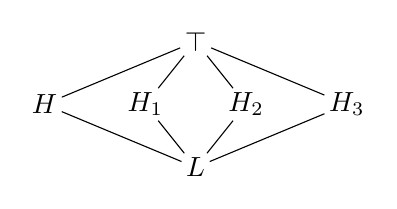
\begin{tikzpicture}[scale=0.8,every node/.style={inner sep=1.5pt}]
      \node (L) at (0,0) {$L$};
      \node (Hh) at (-2.4,1.0) {$H$};
      \node (H1) at (-0.8,1.0) {$H_1$};
      \node (H2) at (0.8,1.0) {$H_2$};
      \node (H3) at (2.4,1.0) {$H_3$};
      \node (T) at (0,2.0) {$\top$};
      \foreach \x in {Hh,H1,H2,H3} {\draw (L) -- (\x); \draw (\x) -- (T);}
    \end{tikzpicture}
  \end{center}
  %(The top level only ensures that $(\Lattice, \sqsubseteq)$ is a semilattice; no
  %program below reads from or writes to the channel $\top$.)

  We reuse the elements of $\Lattice$ as channel names and set
  $\forall \ell.~\gamma(\ell) = \ell^L$, thus giving all channels a low presence label.
  
  Consider the following programs $\PA$ and $\PB$ and states $\sA$ and $\sB$, where
  $\oplus$ denotes exclusive or and all variables are boolean:
  \begin{align*}
    \PA =~& \pIn{H}{r}; & \PB =~ & (\pComp{\pAssign{x'}{0}}{\pAssign{x'}{1}}); \\
        &(\pComp{\pAssign{x}{0}}{\pAssign{x}{1}}); && \pOut{H_2}{\neg x'};\\
        &\pOut{H_1}{\neg x}; && \pIn{H_1}{y'}; \\
        & \pIn{H_2}{y}; && \pOut{H_3}{x' \oplus y'} \\
          & \pOut{H_3}{r \oplus x \oplus y} \\
    \sA =~& \lbrace r = 0, x = 0, y = 0\rbrace & \sB =~& \lbrace x' = 0, y' = 0\rbrace.
  \end{align*}

  Before turning to the formal argument, let us explain the construction. Each program masks its
  contribution to $H_3$ with a fresh bit drawn non-deterministically ($x$ in $\PA$, $x'$ in $\PB$),
  and discloses that mask on a channel ($H_1$, resp.\ $H_2$) invisible at $H_3$. In isolation the
  mask cannot be cancelled, because the user who feeds the program its input---the user of $H_2$
  for $\PA$, of $H_1$ for $\PB$---is not cleared to observe the mask: $H_1 \not\sqsubseteq H_2$ and
  $H_2 \not\sqsubseteq H_1$. In the composition, however, each program plays exactly the role of
  that user for the other one: $\PB$ reads on $H_1$ the mask disclosed by $\PA$, and $\PA$ reads on
  $H_2$ the mask disclosed by $\PB$. The two masks then cancel in the sum of the two outputs on
  $H_3$, which is thereby forced to reveal the secret bit $r$.

  We first show that $\sA \in \StratNI$.

  Since $\gamma(\ell') = {\ell'}^L$ for every channel $\ell'$ and $L \sqsubseteq \ell$ for every
  $\ell \in \Lattice$, the projection $\pi_\ell$ retains \emph{every} label of a trace and hides
  exactly the values carried by channels $\ell' \not\sqsubseteq \ell$. For the same reason,
  $\omega_1 =_\ell \omega_2$ yields, for every channel $\ell'$ and every $t$,
  \begin{align*}
    (*)~~& {\omega_1}_{\ell'}(t) \doteq {\omega_2}_{\ell'}(t), \text{ and}\\
    (**)~~& {\omega_1}_{\ell'}(t) = {\omega_2}_{\ell'}(t) \text{ if moreover } \ell' \sqsubseteq \ell.
  \end{align*}

  Let $\ell \in \Lattice$, $\omega_1 =_\ell \omega_2$, and $\omega_1 \vDash \sA \xrightarrow{t_1}$.
  Then $t_1$ is a prefix of
  $$H?r.H_1!(\neg x).H_2?y.H_3!(r \oplus x \oplus y)$$
  for some choice of $r$, $x$, $y$. We build a run of $\sA$ under $\omega_2$ of the same length;
  as the construction proceeds label by label, it suffices to treat the longest case. Two
  observations drive it:
  \begin{enumerate}[(1)]
  \item Suppose $\PA$ is about to read on a channel $\ell'$, $u_1$ being the prefix of $t_1$
    consumed so far and $u_2$ the prefix of the new run built so far. Then $u_1 =_L u_2$: the two
    carry the same labels, and every channel occurring in them---$H$, $H_1$, $H_2$, $H_3$---is
    $\not\sqsubseteq L$, so $\pi_L$ hides all their values.
    If $\ell' \sqsubseteq \ell$, then also $u_1 =_{\ell'} u_2$, because
    the values we have changed so far all sit on channels $\not\sqsubseteq \ell$ and hence
    $\not\sqsubseteq \ell'$; so ${\omega_1}_{\ell'}(u_1) = {\omega_2}_{\ell'}(u_2)$ by $(**)$ and
    the very same value may be read. If $\ell' \not\sqsubseteq \ell$, then
    ${\omega_1}_{\ell'}(u_1) \doteq {\omega_2}_{\ell'}(u_2)$ by $(*)$, so \emph{some} value may be
    read, and that value is hidden at $\ell$.
  \item The bit $x$ is chosen non-deterministically and is therefore unconstrained by $\omega_2$.
  \end{enumerate}

  If $H_3 \not\sqsubseteq \ell$, we keep the same $x$ and use (1) at the two inputs. Each label of
  the resulting run $t_2$ is then $\ell$-equivalent to the corresponding label of $t_1$: the output
  on $H_1$ carries the same value $\neg x$, and the value output on $H_3$ is hidden at $\ell$.

  If $H_3 \sqsubseteq \ell$, then, since $H,H_1,H_2,H_3$ are pairwise incomparable, either
  $\ell = \top$ or $\ell = H_3$. If $\ell = \top$, then $\omega_1 =_\top \omega_2$ forces
  ${\omega_1}_{\ell'} = {\omega_2}_{\ell'}$ for every channel $\ell'$, and $t_2 = t_1$ satisfies
  the conclusion. If $\ell = H_3$, then $H, H_1, H_2 \not\sqsubseteq H_3$, so $r$, $\neg x$ and $y$
  are all hidden and only the value output on $H_3$ is visible. By (1) we may read some
  $r_2 \in {\omega_2}_H(\varepsilon)$ and, after the output on $H_1$, some $y_2$. Crucially,
  ${\omega_2}_{H_2}$ cannot depend on the value output on $H_1$: since $H_1 \not\sqsubseteq H_2$,
  two traces differing only in that value are $H_2$-equivalent, and $\omega_2$ is a strategy.
  Hence $y_2$ does not depend on the choice of $x$, and (2) lets us set
  $$x_2 = x \oplus r \oplus r_2 \oplus y \oplus y_2,$$
  which gives $r_2 \oplus x_2 \oplus y_2 = r \oplus x \oplus y$ and therefore $t_1 =_{H_3} t_2$.

  The proof that $\sB \in \StratNI$ is similar.

  Now, let $\omega_1$ and $\omega_2$ be any two functions such that
  \begin{align*}
    {\omega_1}_{\ell}(t) = {\omega_2}_{\ell}(t) &= \lbrace v \mid \ell ! v \in t \rbrace && \ell \in \{H_1,H_2\}\\
    {\omega_1}_H(t) &= \{0\} \\
    {\omega_2}_H(t) &= \{1\},
  \end{align*}
  and ${\omega_1}_{\ell} = {\omega_2}_{\ell}$ for $\ell \in \{L,H_3,\top\}$. Neither program reads
  on the latter three channels, so the values taken there are immaterial; setting
  ${\omega_i}_{\ell}(t) = \emptyset$ will do.

  The functions $\omega_1$ and $\omega_2$ are strategies. Since the output of ${\omega_i}_{\ell}$ is constant
  for $i \in \{0,1\}$, $\ell \in \{L,H,H_3,\top\}$, the only interesting case is when $\ell \in \{H_1,H_2\}$.
  W.l.o.g., consider $\omega_1$ and $H_1$, for which we have $\gamma(H_1) = H_1^L$. If $t_1 =_{H_1} t_2$,
  then in particular $\lbrace v \mid H_1!v  \in t_1\rbrace = \lbrace v \mid H_1! v \in t_2\rbrace$.
  If $t_1 =_L t_2$, then $H_1 ! v \in t_1$ (resp. $H_1 ! v \in t_2$) implies the existence of some $H_1 ! v' \in t_2$
  (resp. $H_1 ! v' \in t_1$), and  hence $\lbrace v \mid H_1!v  \in t_1\rbrace \doteq \lbrace v \mid H_1! v \in t_2\rbrace$.

  Furthermore, we have $\omega_1 =_{H_3} \omega_2$. Namely, ${\omega_1}_{\ell}(t) = {\omega_2}_{\ell}(t)$
  for all $t$ and all $\ell \sqsubseteq H_3$, i.e. $\ell \in \{L, H_3\}$,
  and, for all $\ell$, $t$, we can immediately verify that ${\omega_1}_{\ell}(t)\doteq {\omega_2}_{\ell}(t)$.

  We introduce the following trace $t$:
  $$t = H?0.H_1!0.H_2!0.H_2?0.H_1?0.H_3!1.H_3!1.$$

  Next, we show that $\omega_1 \vDash \sA \parallel \sB \xrightarrow{t}$ but there is no $t' =_{H_3} t$ such that
  $\omega_2 \vDash \sA \parallel \sB \xrightarrow{t'}$. This will conclude the proof that $\sA \parallel \sB \notin \StratNI$.

  The fact that $\omega_1 \vDash \sA \parallel \sB \xrightarrow{t}$ is easily verified by running the above
  programs concurrently with non-determinism $x := 1$, $x' := 1$. Any interleaving that executes the two outputs to $H_1$ and $H_2$
  before the two inputs from $H_1$ and $H_2$ can be chosen. The output of $\PA$ to $H_1$ is read
  by $\PB$ into $y'$, and the output of $\PB$ to $H_2$ is read by $\PA$  into $y$.

  Assume towards a contradiction that we have some $t'$ fulfilling $t' =_{H_3} t$
  and $\omega_2 \vDash \sA \parallel \sB \xrightarrow{t'}$. Since $t' =_{H_3} t$, $t'$ must
  be of the form
  $$t' = H?r.H_1!a.H_2!b.H_2?c.H_1?d.H_3!1.H_3!1,$$
  and by $\omega_2 \vDash \sA \parallel \sB \xrightarrow{t'}$, we additionally know that $r = 1$.
  A trace of the above form can only be obtained when running both programs to the end. In
  particular, the two outputs must be performed before the two inputs, and, since at most
  one output is performed to each of $H_1$ and $H_2$, it must be the case that $a = d$ and $b = c$.
  One of the outputs to $H_3$ is $r \oplus x \oplus y = r \oplus (\neg a) \oplus b$, performed
  by $\PA$. The other output to $H_3$ is $x' \oplus y' = a \oplus (\neg b)$, performed by $\PB$.
  Hence, the exclusive or of the two inputs must be $(r \oplus (\neg a) \oplus b) \oplus (a \oplus (\neg b))=r$. But since $1 \oplus 1 = 0$, this contradicts $r = 1$. Hence, such a $t'$ does
  not exist, and $\sA \parallel \sB \notin \StratNI$.
  
\end{proof}

The construction above makes essential use of colluding observers with
uncomparable levels. Collusion is a known issue in the security of nondeterministic
systems, and can be addressed by introducing properties that consider \emph{coalitions}
of observers~\cite{Engelhardt2012,Muller2018}\footnote{We are indebted to the anonymous referee for this suggestion.}.
Accordingly, we define:


\begin{definition}[CINI]
  \label{def:coalition}
  A \emph{coalition} is a set of levels $C \subseteq \Lattice$.
  Write $\Lattice^* := \Pow{\Lattice}$ and, for $C, D \in \Lattice^*$
  and $\alpha \in \Channels$ with $\gamma(\alpha) = \ell_1^{\ell_2}$,
  \begin{align*}
    C \sqsubseteq^* D &\overset{\mathrm{def.}}{\Longleftrightarrow} \forall c \in C.~\exists d \in D.~c \sqsubseteq d; &
    \gamma^*(\alpha) &\overset{\mathrm{def.}}{=} \{\ell_1\}^{\{\ell_2\}}.
  \end{align*}
  Then $(\Lattice^*, \sqsubseteq^*)$ is a semilattice
  and $(\Lattice^*, \sqsubseteq^*, \gamma^*)$ is a security context
  in the sense of Section~\ref{sec:preliminaries}.
  For any $W \subseteq \Strat$, a state $s$ is \emph{$W$-coalition-noninterfering} iff, for
  all $C \in \Lattice^*$, $\omega_1,\omega_2 \in W$, and $t_1 \in \Traces$,
  \begin{align*}
    \omega_1 =_C \omega_2 \Longrightarrow \omega_1 \models s \xrightarrow{t_1}\,\Longrightarrow
    \exists t_2.\,\omega_2 \models s \xrightarrow{t_2} \land\, t_1 =_C t_2.
  \end{align*}
  We then write $s \in W\text{-NI}^*$.
  \leanref{Sec.coalition}
\end{definition}

Since $\{\ell\} \sqsubseteq^* \{\ell'\}$ iff $\ell \sqsubseteq \ell'$, CINI implies INI.
CINI is a strictly stronger notion:

\begin{theorem}
  \label{thm:coalition rejects}
  $\sA \in \StratNI$, but $\sA \notin \StratNI^*$.
  \leanref{Cex1.coalitionNI\_strictly\_stronger}
\end{theorem}
\begin{proof}
  Take $C = \{H_1, H_3\}$: the user to whom $\PA$ discloses its mask, together with the observer to
  whom it delivers its output. Let $\omega_1$ and $\omega_2$ agree on every channel except that
  ${\omega_1}_H(t) = \{0\}$ and ${\omega_2}_H(t) = \{1\}$, with ${\omega_i}_{H_2}(t) = \{0\}$. Then
  $\omega_1 =_C \omega_2$, since $\{H\} \not\sqsubseteq^* C$ and $\{H_2\} \not\sqsubseteq^* C$,
  while all presence levels are $L$. Under $\omega_1$, $\PA$ can produce
  $H?0.H_1!(\neg x).H_2?0.H_3!x$; under $\omega_2$, every run produces
  $H?1.H_1!(\neg x_2).H_2?0.H_3!(\neg x_2)$. Both the value on $H_1$ and the value on $H_3$ are
  visible to $C$, so a match would require $x_2 = x$ and $\neg x_2 = x$.
\end{proof}

Theorem~\ref{thm:noncompositional} thus refutes \cite[Theorem V.1]{Rafnsson2012} as stated, for
arbitrary lattices; compositionality \emph{is} restored under the stronger notion of
Definition~\ref{def:coalition}, as Section~\ref{sec:coalition composes} shows.

\subsection{Analysis of the previously published proofs}
\label{sec:flawed proof}

In a paper published at CSF'12, Rafnsson et al. claim to
have proven the compositionality of reactive non-interference~\cite[p. 301-302]{Rafnsson2012}.
Unfortunately, the published proof is incorrect.
Given two states $\sA, \sB \in \StratNI$,
an execution $\omega_1 \vDash \sA \parallel \sB \xrightarrow{t_1}$, and $\omega_2 =_\ell \omega_1$, the authors try to construct
$t_2 =_\ell t_1$ such that $\omega_2 \vDash \sA \parallel \sB \xrightarrow{t_2}$. Their proof attempt proceeds in three
steps:
\begin{enumerate}
\item They decompose $t_1$ in an interleaving of two traces $t_{1\mathtt{A}}$ and $t_{1\mathtt{B}}$ corresponding
  to the inputs and outputs caused by the execution of the two subprograms.
\item Using $\omega_1$ and $\omega_2$,
  they define strategies $\omega_{1\mathtt{A}}$, $\omega_{1\mathtt{B}}$, $\omega_{2\mathtt{A}}$, and $\omega_{2\mathtt{B}}$
  for which they claim that $\omega_{1k} =_\ell \omega_{2k}$ for $k \in \{\mathtt{A},\mathtt{B}\}$, and then use
  the noninterference property of $\sA$ and $\sB$ to obtain $t_{2\mathtt{A}} =_\ell t_{1\mathtt{A}}$ and $t_{2\mathtt{B}} =_\ell t_{1\mathtt{B}}$.
\item They obtain $t_2$ such that $t_2 =_\ell t_1$ and $\omega_2 \vDash \sA \parallel \sB \xrightarrow{t_2}$ by
  interleaving $t_{2\mathtt{A}}$ and $t_{2\mathtt{B}}$.
\end{enumerate}
The proof of $\omega_{1k} =_\ell \omega_{2k}$ in step (2) contains a mistake. The authors claim that, for some $t'_1$,
$\alpha$, and $v$ such that $\gamma(\alpha)=\ell_1^{\ell_2}$ and $\ell_1 \sqsubseteq \ell$,
the two assumptions $\omega_1 \vDash \sA \parallel \sB \xrightarrow{t'_1.\alpha?v}$ and $\omega_1 =_\ell \omega_2$ 
imply $\omega_2 \vDash \sA \parallel \sB \xrightarrow{t'_1.\alpha?v}$. This implication cannot be proven from the
assumptions; in fact, it appears to be a stronger form of the proof goal
\begin{align*}
  \forall t_1.~&\omega_1 \vDash \sA \parallel \sB \xrightarrow{t_1}\Longrightarrow \exists t_2.~t_2 =_\ell t_1 \wedge \omega_2 \vDash \sA \parallel \sB \xrightarrow{t_2}
\end{align*}
and thus introduces a circular argument. A similar flaw is found in the case $\ell_1 \not\sqsubseteq \ell \wedge \ell_2 \sqsubseteq \ell$.

%We identified a very similar logical flaw in a proof of a related notion of noninterference for component-based systems published
%by Greiner et al.~\cite[p. 265]{Greiner2016} at CSF'16, which is also included in a PhD thesis~\cite[p. 31-33]{Greiner2018}.
%While the counterexample described in this paper may not directly apply to Greiner et al.'s work, the very similar proof patterns
%suggest that further work may be needed to guarantee the correctness of the results claimed.

\subsection{Non-compositionality for total strategies}

We now extend the attack described at the beginning of this section to total strategies. This corresponds to the
setup described in O'Neill et al.'s original paper~\cite{ONeill2006}.

\begin{theorem}[Non-compositionality for total strategies]
  \label{thm:noncompositional total}
  There exists $\sA,\sB \in \StratTNI$ such that $\sA \parallel \sB \notin \StratTNI$.
  \leanref{noncompositional\_total}
\end{theorem}
\begin{proof}
  Let $(\Lattice, \sqsubseteq)$ be the lattice with $\Lattice = \lbrace L_1, L_2, H, H_1, H_2, H_3, \top \rbrace$
  and $\sqsubseteq = \lbrace (L_i, \ell) \mid i \in \{1,2\},\ell \in \Lattice\rbrace \cup \lbrace (\ell, \ell) \mid \ell \in \Lattice\rbrace
  \cup \lbrace (\ell, \top) \mid \ell \in \Lattice\rbrace$, i.e.,
  the $H_j$-levels and $H$ are pairwise incomparable, the $L_i$ are lower and $\top$ higher than all
  other levels; the Hasse diagram is the one above with $L$ replaced by the two mutually
  $\sqsubseteq$-equivalent bottom levels $L_1$ and $L_2$, which serve only to provide two distinct
  public channels. As before we reuse the levels as channel names, and, since presence is always
  public in the total setup, we set $\forall \ell.~\gamma(\ell) = \ell^{L_1}$.
  Consider the following programs and states, with new code in blue:
  \begin{align*}
    \PA =~& \pIn{H}{r}; & \PB =~ & (\pComp{\pAssign{x'}{0}}{\pAssign{x'}{1}}); \\
          &(\pComp{\pAssign{x}{0}}{\pAssign{x}{1}}); && \pOut{H_2}{\neg x'};\\
          &\pOut{H_1}{\neg x}; && {\color{blue} \pOut{L_2}{1};} \\
          &{\color{blue}\pOut{L_1}{1};} && {\color{blue}\pIn{L_1}{z'};} \\
          &{\color{blue}\pIn{L_2}{z};} && \pIn{H_1}{y'}; \\
          &\pIn{H_2}{y}; && {\color{blue}\pOut{H_3}{z'};}\\
          &{\color{blue}\pOut{H_3}{z};} && \pOut{H_3}{x' \oplus y'} \\
          &\pOut{H_3}{r \oplus x \oplus y} \\
    \sA =~& \lbrace r = 0, x = 0, y = 0\rbrace & \sB =~& \lbrace x' = 0, y' = 0\rbrace.
  \end{align*}
  The proof that $\sA,\sB \in \StratTNI$ is similar to before, observing that any $t_1$ for
  which $\omega_1 \vDash \sA \xrightarrow{t_1}$ is prefix of
  $$H?r.H_1!(\neg x).L_1!1.L_2?z.H_2?y.H_3!z.H_3!(r \oplus x \oplus y)$$
  for some choice of $r$, $x$, $y$, $z$. With total strategies, the output to $L_1$ is
  independent of any input; the data in $z$ is allowed to flow from $L_2$ to $H_3$
  since $L_2 \sqsubseteq H_3$.

  Now, consider the following functions $\omega_1$ and $\omega_2$:
  \begin{align*}
    {\omega_1}_{\ell}(t) = {\omega_2}_{\ell}(t) &= \{0\} && \ell \in \{H_3, \top\}\\
    {\omega_1}_{\ell}(t) = {\omega_2}_{\ell}(t) &= \lbrace v \mid \ell ! v \in t \rbrace && \ell \in \Lambda_t\\
    {\omega_1}_{\ell}(t) = {\omega_2}_{\ell}(t) &= \{0\} && \ell \in \Lambda \setminus \Lambda_t\\
    {\omega_1}_H(t) &= \{0\} \\
    {\omega_2}_H(t) &= \{1\},
  \end{align*}
  where $\Lambda = \{L_1,L_2,H_1,H_2\}$ and
  $\Lambda_t = \{\ell \in \Lambda \mid \exists v.\,\ell!v \in t\}$.
  Just as before, the functions $\omega_1$ and $\omega_2$ are strategies and $\omega_1 =_{H_3} \omega_2$. We now show that the trace
  \begin{align*}
    t &= H?0.H_1!0.L_1!1.H_2!0.L_2!1.L_2?1.H_2?0.L_1?1.H_1?0.\\
      &\quad\,H_3!1.H_3!1.H_3!1.H_3!1.
  \end{align*}
  satisfies $\omega_1 \vDash \sA \parallel \sB \xrightarrow{t}$, while
  $\omega_2 \vDash \sA \parallel \sB \xrightarrow{t'}$ holds for no $t' =_{H_3} t$.

  The first point is obtained as before, running $\PA$ with $x := 1$ and $\PB$ with $x' := 1$.
  The programs are interleaved as follows: $\PA$ first reads $r=0$ from $H$ and outputs $\neg x=0$
  to $H_1$ and $1$ to $L_1$; then $\PB$ outputs $\neg x'=0$ to $H_2$ and $1$ to $L_2$; next
  $\PA$ reads $z=1$ from $L_2$ and $y=0$ from $H_2$,
  and $\PB$ reads $z'=1$ from $L_1$ and $y'=0$ from $H_1$;
  finally, $\PA$ outputs $z=1$ and $r \oplus x \oplus y=1$ to $H_3$ and $\PB$ outputs $z'=1$
  and $x' \oplus y'=1$ to $H_3$. Hence $\omega_1 \vDash \sA \parallel \sB \xrightarrow{t}$.

  Assume towards a contradiction that we have some $t'$ fulfilling $t' =_{H_3} t$
  and $\omega_2 \vDash \sA \parallel \sB \xrightarrow{t'}$. Since $t' =_{H_3} t$, $t'$ must
  be of the form
  \begin{align*}
    t' &= H?r.H_1!a.L_1!1.H_2!b.L_2!1.L_2?1.H_2?c.L_1?1.H_1?d.\\
      &\quad\,H_3!1.H_3!1.H_3!1.H_3!1,
  \end{align*}
  and by $\omega_2 \vDash \sA \parallel \sB \xrightarrow{t'}$ we have $r=1$.
  Since the four outputs to $H_3$ are $1$, we know that the two programs have been executed
  to the end and that the two $\pOut{L_i}{1}$ have been executed before 
  $\pIn{L_1}{z'}$ and $\pIn{L_2}{z}$. Given the order of inputs and outputs in $\PA$ and $\PB$,
  this implies that $\pOut{H_1}{\neg x}$ and $\pOut{H_2}{\neg x'}$ have been executed
  before $\pIn{H_1}{y'}$ and $\pIn{H_2}{y}$. As a consequence, $a=d$ and $b=c$. The conclusion
  is as in the non-total case.  
\end{proof}

\section{Compositionality in the deterministic case}

\label{sec:deterministic}

The counterexamples presented in the previous section crucially depend on programs being non-deterministic.
In these countereamples, each individual program uses a non-deterministic choice to make an output
distributionally independent of an input; however, since pairs of independent variables can be correlated between them,
this form of `hiding through independence' is not preserved through composition.
In this section, we show that imposing determinism on individual programs recovers compositionality.
Note that determinism is required of the \emph{composed programs} only:
the \emph{composition} of two deterministic programs is still non-deterministic in general,
since it retains the scheduling non-determinism of the interleaving.

In every statement below, $\ell$ ranges over $\Lattice$ and is universally quantified. We first
isolate the two transformations of strategies used by the proofs and prove helper lemmata.

\subsection{Two strategy transformations}

For any channel $\alpha$ and trace $t$, write $t \setminus \alpha$ for the trace obtained from $t$
by deleting its first label on channel $\alpha$ (and $t \setminus \alpha = t$ if $t$ contains no
such label). For any $D \subseteq \Values$, let $\omega[\alpha \mapsto D]$ be given by
\begin{align*}
  {\omega[\alpha \mapsto D]}_{\alpha'}(t) &= D && \hspace{-1.2em}\text{if } \alpha' = \alpha, \alpha \text{ not in } t\\
  {\omega[\alpha \mapsto D]}_{\alpha'}(t) &= {\omega}_{\alpha'}(t \setminus \alpha) && \hspace{-1.2em}\text{otherwise;}
\end{align*}
and, for any trace $u$, let $u \triangleright \omega$ be given by
${(u \triangleright \omega)}_{\alpha'}(t) = \omega_{\alpha'}(u.t)$.
Intuitively, $\omega[\alpha \mapsto D]$ is $\omega$ \emph{delayed} by one step on $\alpha$, while
$u \triangleright \omega$ is $\omega$ \emph{advanced} past the prefix $u$. In both cases the
transformation applies to \emph{all} channels $\alpha'$, and not only to $\alpha$: this is
essential, since one step of the program shifts the history seen by every user.

Let $\gamma(\alpha) = \ell_1^{\ell_2}$. For any level $m$, $\pi_m(t \setminus \alpha)$ is obtained
from $\pi_m(t)$ by deleting its first entry on $\alpha$ if $\ell_2 \sqsubseteq m$, and
$\pi_m(t\setminus\alpha) = \pi_m(t)$ otherwise; likewise, whether $\alpha$ occurs in $t$ is
determined by $\pi_m(t)$ whenever $\ell_2 \sqsubseteq m$. Since $\ell_2 \sqsubseteq \ell_1$, it
follows that:
\begin{enumerate}[(i)]
\item $\omega[\alpha \mapsto D]$ is again a strategy;
\item ${\omega[\alpha \mapsto D]}_{\alpha'}(\alpha : v.t) = {\omega}_{\alpha'}(t)$ for all $\alpha'$, $v$, $t$;
\item if $\omega_1 =_\ell \omega_2$, $D_1 \doteq D_2$, and $\ell_1 \sqsubseteq \ell$ implies
  $D_1 = D_2$, then $\omega_1[\alpha \mapsto D_1] =_\ell \omega_2[\alpha \mapsto D_2]$.
\end{enumerate}
Since $=_m$ is a congruence for concatenation, we obtain similarly:
\begin{enumerate}[(i)]\setcounter{enumi}{3}
\item $u \triangleright \omega$ is again a strategy;
\item if $u =_\ell u'$ and $\omega_1 =_\ell \omega_2$, then
  $u \triangleright \omega_1 =_\ell u' \triangleright \omega_2$.
\end{enumerate}
For (v), note that $\ell_1 \sqsubseteq \ell$ implies $u =_{\ell_1} u'$, whence
${\omega_1}_{\alpha}(u.t) = {\omega_1}_{\alpha}(u'.t) = {\omega_2}_{\alpha}(u'.t)$, and
symmetrically for $\ell_2$ with $\doteq$ instead of $=$.

\subsection{Compositionality}

We now prove a few helper lemmata.
\begin{lemma}
  \label{thm:deterministic step}
  Consider a deterministic IOLTS. If $s \in \StratNI$ and $s \xrightarrow{e} s'$, then
  $s' \in \StratNI$.
  \leanref{Sec.deterministic\_step}
\end{lemma}
\begin{proof}
  Let $\omega_1, \omega_2 \in \Strat$, $\ell \in \Lattice$, $\omega_1 =_\ell \omega_2$.
  Assume that $\omega_1 \vDash s' \xrightarrow{t_1}$ for some $t_1$. We want to obtain
  $t_2 =_\ell t_1$ such that  $\omega_2 \vDash s' \xrightarrow{t_2}$. The idea is to prefix the run
  of $s'$ by the step $s \xrightarrow{e} s'$, apply noninterference of $s$, and then strip that step
  off again; the transformation $\omega \mapsto \omega[\alpha \mapsto D]$ performs the required
  adjustment of the strategies, and determinism guarantees that the run obtained from $s$ does
  begin with the same step.

  We do a case distinction on $e$:
  \begin{itemize}
  \item If $e = \tau$, then $\omega_1 \vDash s \xrightarrow{t_1}$. By NI of $s$, we get $t_2 =_\ell t_1$
    such that $\omega_2 \vDash s \xrightarrow{t_2}$. If the latter execution is of length zero, then we have
    $t_2 = \varepsilon$, and we get $\omega_2 \vDash s' \xrightarrow{t_2}$ by running 0 steps from $s'$
    under $\omega_2$. If it is of length at least one, then it starts with $s \xrightarrow{e'} s''$ for some $e'$
    and $s''$. Since $s \xrightarrow{\tau} s'$, clause (i) of Definition~\ref{def:deterministic}
    forces $e' = \tau$, and clause (ii) then forces $s'' = s'$; thus we get
    $\omega_2 \vDash s' \xrightarrow{t_2}$.
  \item If $e = \alpha ! v$, let $\gamma(\alpha) = \ell_1^{\ell_2}$.

    For $i \in \{1,2\}$, we set $\omega'_i = \omega_i[\alpha \mapsto \emptyset]$. By (i) and (iii)
    above, the $\omega'_i$ are strategies and $\omega'_1 =_\ell \omega'_2$.

    Given $\omega_1 \vDash s' \xrightarrow{t_1}$ and $s \xrightarrow{\alpha!v} s'$, the definition of $\omega'_1$
    ensures that $\omega'_1 \vDash s \xrightarrow{\alpha!v.t_1}$.  
    Applying NI of $s$, we get $t'_2 =_\ell \alpha!v.t_1$ such that $\omega'_2 \vDash s \xrightarrow{t'_2}$.
    
    The case $t'_2 = \varepsilon$ is as for $\tau$. 
    Otherwise, $t'_2$ is non-empty. The execution
    of $s$ under $\omega'_2$ must start with a step $s \xrightarrow{e'} s''$, which by determinism must
    be $s \xrightarrow{\alpha!v} s'$. $t'_2$ is of the form $\alpha ! v.t_2$. From $\alpha!v.t_2 =_\ell \alpha!v.t_1$
    we get $t_2 =_\ell t_1$. By the fact that $\omega'_2 \vDash s \xrightarrow{\alpha!v.t_2}$ and the definition
    of $\omega'_2$, we finally obtain $\omega_2 \vDash s' \xrightarrow{t_2}$.
  \item If $e = \alpha ? v$, let $\gamma(\alpha) = \ell_1^{\ell_2}$.

    For $i \in \{1,2\}$, we set $\omega'_i = \omega_i[\alpha \mapsto \{v\}]$. By (i) and (iii)
    above, the $\omega'_i$ are strategies and $\omega'_1 =_\ell \omega'_2$.

    Given $\omega_1 \vDash s' \xrightarrow{t_1}$ and $s \xrightarrow{\alpha?v} s'$, the definition of $\omega'_1$
    ensures that $\omega'_1 \vDash s \xrightarrow{\alpha?v.t_1}$.  
    Applying NI of $s$, we get $t'_2 =_\ell \alpha?v.t_1$ such that $\omega'_2 \vDash s \xrightarrow{t'_2}$.
    
    The case $t'_2 = \varepsilon$ is as for $\tau$. 
    Otherwise, $t'_2$ is non-empty. The execution
    of $s$ under $\omega'_2$ must start with a step $s \xrightarrow{e'} s''$, which by determinism must
    be $s \xrightarrow{\alpha?v'} s'$ for some $v'$. By definition of $\omega'_2$, we get $v'=v$.
    Now, $t'_2$ is of the form $\alpha ? v.t_2$. From $\alpha?v.t_2 =_\ell \alpha?v.t_1$
    we get $t_2 =_\ell t_1$, and, by $\omega'_2 \vDash s \xrightarrow{\alpha?v.t_2}$ and the definition
    of $\omega'_2$, we conclude that $\omega_2 \vDash s' \xrightarrow{t_2}$.
  \end{itemize}
  
\end{proof}

The next lemma is the key of the compositionality proof. It lifts noninterference from a
single state to a \emph{pair} of states reached from a noninterfering state by $\ell$-equivalent
histories: whatever a component can do from $\sC$ under $\omega_1$ can be matched from $\sE$ under
$\omega_2$.

\begin{lemma}
  \label{thm:indistinguishable NI}
  Consider a deterministic IOLTS. If
    \begin{gather*}
    \sA \in \StratNI \quad
    \omega_1,\omega_2 \in \Strat\\
    \sA \xrightarrow{t} \sC \quad
    \sA \xrightarrow{t'} \sE\quad
    \omega_1 \vDash \sC \xrightarrow{t_1} \quad
    t =_\ell t'\quad
    \omega_1 =_\ell \omega_2
  \end{gather*}
  then there exists $t_2 =_\ell t_1$ such that $\omega_2 \vDash \sE \xrightarrow{t_2}$.
  \leanref{Sec.indistinguishable\_NI}
\end{lemma}
\begin{proof}
  For any trace $u$, define the strategy $\omega \setminus u$ by iterating the construction of the
  previous lemma along $u$:
  $$\omega \setminus \varepsilon = \omega, \qquad
  \omega \setminus (\alpha : v.u) = (\omega \setminus u)[\alpha \mapsto D_{\alpha:v}],$$
  where $D_{\alpha ? v} = \{v\}$ and $D_{\alpha ! v} = \emptyset$. By (i) above, $\omega\setminus u$
  is a strategy. Two straightforward inductions on $u$, resp. on $|u| + |u'|$, using (ii), resp. (iii),
  give:
  \begin{enumerate}[(a)]
  \item if $s \xrightarrow{u} s''$ and $\omega \vDash s'' \xrightarrow{r}$, then
    $\omega \setminus u \vDash s \xrightarrow{u.r}$;
  \item if $u =_\ell u'$ and $\omega_1 =_\ell \omega_2$, then
    $\omega_1 \setminus u =_\ell \omega_2 \setminus u'$.
  \end{enumerate}
  For (b), note that a label $\alpha : v$ with $\ell_2 \not\sqsubseteq \ell$ can be dropped on either
  side by (iii) (as then $\ell_1 \not \sqsubseteq \ell$), while two labels that are visible at $\ell$
  agree on their channel, on their direction, and---if $\ell_1 \sqsubseteq \ell$---on their value.

  By (a), $\omega_1 \setminus t \vDash \sA \xrightarrow{t.t_1}$, and by (b),
  $\omega_1 \setminus t =_\ell \omega_2 \setminus t'$. Applying $\sA \in \StratNI$, we obtain
  $\hat{t}_2 =_\ell t.t_1$ such that $\omega_2 \setminus t' \vDash \sA \xrightarrow{\hat{t}_2}$.

  By determinism and by construction of $\omega_2 \setminus t'$, every run of $\sA$ consistent with
  $\omega_2 \setminus t'$ follows the execution $\sA \xrightarrow{t'} \sE$: an induction on the latter
  shows that either (1) $t'$ is of the form $\hat{t}_2.\hat{u}$, or (2) $\hat{t}_2$ is of the form
  $t'.t_2$ with $\omega_2 \vDash \sE \xrightarrow{t_2}$.

  In case (2), $\pi_\ell(t).\pi_\ell(t_1) = \pi_\ell(\hat{t}_2) = \pi_\ell(t').\pi_\ell(t_2)$, and
  $t =_\ell t'$ gives $t_1 =_\ell t_2$, as required. In case (1), $\pi_\ell(\hat{t}_2)$ is a prefix of
  $\pi_\ell(t') = \pi_\ell(t)$ and equals $\pi_\ell(t).\pi_\ell(t_1)$; hence
  $\pi_\ell(t_1) = \varepsilon$ and $t_2 = \varepsilon$ satisfies the conclusion.
\end{proof}

\begin{theorem}
  \label{thm:helper deterministic}
  Consider a deterministic IOLTS. If
  \begin{gather*}
    \sA, \sB, \sC, \sD, \sE, \sF \in \StratNI\quad
    \omega_1,\omega_2 \in \Strat\\
    \sA \xrightarrow{t_{\mathtt{A}}} \sC \quad \sA \xrightarrow{t'_{\mathtt{A}}} \sE\quad
    \sB \xrightarrow{t_{\mathtt{B}}} \sD \quad \sB \xrightarrow{t'_{\mathtt{B}}} \sF\\
    \omega_1 \vDash \sC \parallel \sD \xrightarrow{t_1} \quad
    t_{\mathtt{A}} =_\ell t'_{\mathtt{A}} \quad t_{\mathtt{B}} =_\ell t'_{\mathtt{B}}\quad
    \omega_1 =_\ell \omega_2
  \end{gather*}
  then there exists $t_2 =_\ell t_1$ such that $\omega_2 \vDash \sE \parallel \sF \xrightarrow{t_2}$.
  \leanref{Sec.compose\_helper}
\end{theorem}
\begin{proof}
  By induction on the length of the execution $\sC \parallel \sD \xrightarrow{t_1}$. The induction
  hypothesis is the statement of the theorem itself, for all strictly shorter executions and all
  instantiations of its parameters---in particular of $\sC,\sD,\sE,\sF$, of
  $t_{\mathtt{A}},t'_{\mathtt{A}},t_{\mathtt{B}},t'_{\mathtt{B}}$, and of $\omega_1,\omega_2$.

  If this execution is empty, then $t_1 = \varepsilon$ and choosing $t_2 = \varepsilon$
  yields the conclusion.

  Otherwise, the execution can be decomposed, w.l.o.g., as $\sC \xrightarrow{e} \sC'$, $\sC' \parallel \sD \xrightarrow{t_1'}$. 
  \begin{itemize}
  \item If $e = \tau$, then, since silent steps leave no mark on traces, $\sA \xrightarrow{t_{\mathtt{A}}} \sC$
    and $\sC \xrightarrow{\tau} \sC'$ give $\sA \xrightarrow{t_{\mathtt{A}}} \sC'$, and the remainder
    of the execution witnesses $\omega_1 \vDash \sC' \parallel \sD \xrightarrow{t_1}$ with the same
    trace $t_1$ and a strictly shorter execution. Furthermore, by
    Lemma~\ref{thm:deterministic step}, we have $\sC' \in \StratNI$.
    Hence, by IH, we get $t_2 =_\ell t_1$ such
    that $\omega_2 \vDash \sE \parallel \sF \xrightarrow{t_2}$.

  \item If $e = \alpha:v$, we have $t_1 = \alpha:v.t'_1$.

    First, observe that
    $\omega_1 \vDash \sC \xrightarrow{e}$ and
    $\forall t'_2,\sE'.~\omega_2 \vDash \sE \xrightarrow{t_2'} \sE' \Longrightarrow \omega_2 \vDash \sE \parallel \sF \xrightarrow{t_2'} \sE' \parallel \sF$.

    Since $\sA \in \StratNI$, $\sA \xrightarrow{t_{\mathtt{A}}} \sC$, $\sA \xrightarrow{t'_{\mathtt{A}}} \sE$,
    and $t_{\mathtt{A}} =_\ell t'_{\mathtt{A}}$, then by Lemma~\ref{thm:indistinguishable NI} there
    exists $t'' =_\ell \alpha:v$ and $\sE'$ such that
    $\omega_2 \vDash \sE \xrightarrow{t''} \sE'$,  and therefore
    $\omega_2 \vDash \sE \parallel \sF \xrightarrow{t''} \sE' \parallel \sF$.

    Set $\omega'_1 = (\alpha\!:\!v) \triangleright \omega_1$ and $\omega'_2 = t'' \triangleright \omega_2$.
    By (iv) both are strategies, and, since $\alpha\!:\!v =_\ell t''$ and $\omega_1 =_\ell \omega_2$,
    property (v) gives $\omega'_1 =_\ell \omega'_2$.

    Finally, we observe that the definition of $\omega'_1$ and the fact that $\omega_1 \vDash \sC \parallel \sD \xrightarrow{t_1}$
    has the first step $\sC \xrightarrow{\alpha:v} \sC'$  ensure $\omega'_1 \vDash \sC' \parallel \sD \xrightarrow{t'_1}$.

    Now, by Lemma~\ref{thm:deterministic step}, $\sC', \sE' \in \StratNI$; furthermore,
    $\omega'_1,\omega'_2 \in \Strat$,
    $\sA \xrightarrow{t_{\mathtt{A}}.\alpha:v} \sC'$, $\sA \xrightarrow{t'_{\mathtt{A}}.t''} \sE'$,
    $\sB \xrightarrow{t_{\mathtt{B}}} \sD$, $\sB \xrightarrow{t'_{\mathtt{B}}} \sF$,
    $\omega'_1 \vDash \sC' \parallel \sD \xrightarrow{t'_1}$,
    $t_{\mathtt{A}}.\alpha:v =_\ell t'_{\mathtt{A}}.t''$, $t_{\mathtt{B}} =_\ell t'_{\mathtt{B}}$,
    and $\omega'_1 =_\ell \omega'_2$.
    By IH, we get $t'_2 =_\ell t'_1$ such that
    $\omega'_2 \vDash \sE' \parallel \sF \xrightarrow{t'_2}$. Hence, $\alpha:v.t'_1 =_\ell t''.t'_2$
    and the definition of $\omega'_2$ ensures that $\omega_2 \vDash \sE \parallel \sF \xrightarrow{t''.t'_2}$.
  \end{itemize}
\end{proof}

Finally, we prove compositionality of INI for deterministic programs:

\begin{theorem}
  \label{thm:deterministic}
  Consider a deterministic IOLTS. If $\sA, \sB \in \StratNI$, then $\sA \parallel \sB \in \StratNI$.
  \leanref{Sec.deterministic\_compositional}
\end{theorem}
\begin{proof}
  Immediate from Theorem~\ref{thm:helper deterministic}, setting $\sC = \sE = \sA$, $\sD = \sF = \sB$,
  and $t_{\mathtt{A}} = t'_{\mathtt{A}} = t_{\mathtt{B}} = t'_{\mathtt{B}} = \varepsilon$.
\end{proof}

An IOLTS obtained by parallel composition is, in general, no longer deterministic: as soon as both
components can move, the composition has two distinct steps carrying different labels, which
violates clause (i) of Definition~\ref{def:deterministic}. Theorem~\ref{thm:deterministic} can
therefore \emph{not} be applied iteratively, as $\sA \parallel \sB$ is not a legal argument for a
second application. Fortunately, the hypotheses of Theorem~\ref{thm:helper deterministic} mention
the two components separately, so both it and Theorem~\ref{thm:deterministic} adapt in a
straightforward manner to the composition of an arbitrary---finite or infinite---family of
deterministic IOLTS, each component being required to be deterministic and noninterfering. This
leads to the following theorem:
\begin{theorem}
  \label{thm:deterministic family}
  Consider a family $(s_i)_{i\in I}$ of deterministic IOLTS. If $s_i \in \StratNI$ for all $i \in I$, then $\parallel_{i \in I} s_i \in \StratNI$.
  \leanref{Sec.deterministic\_compositional\_family}
\end{theorem}

\subsection{Consequence for Rafnsson et al.'s type system}

Theorem~\ref{thm:deterministic family} has a direct consequence for the type system that
Rafnsson et al.~\cite{Rafnsson2012} propose to check INI statically. They first give a type system
for deterministic programs, and then extend it to non-determinism by the rule
\begin{align*}
    \frac{\vdash_\gamma p_1 \quad \vdash_\gamma p_2}{\vdash_\gamma p_1 \mid p_2}\textrm{par}
\end{align*}
which types a parallel composition $p_1 \mid p_2$ under a context $\gamma$ iff both $p_1$ and
$p_2$ can be typed under the same context. In their calculus $\mid$ denotes parallel composition,
whereas in our examples it denotes non-deterministic choice; we keep both usages, for consistency
with the respective sources. Since the \textrm{par} rule is the only source of
non-determinism, a type-correct program is, by construction, a parallel composition of finitely
many programs typed in the deterministic fragment---finitely many because programs are finite
syntactic objects. Each of these is deterministic and, by soundness of the deterministic fragment,
noninterferent; Theorem~\ref{thm:deterministic family} then yields noninterference of the whole.
(The infinite case of Theorem~\ref{thm:deterministic family} is needed only for extensions that
admit unboundedly many components, such as unbounded thread creation.)

As a result, Rafnsson et al.'s type system is sound, even in the presence of non-deterministic
programs, despite the gap in the compositionality theorem it was meant to rest on. Using this type
system, however, non-determinism cannot be used \emph{to achieve} noninterference; for instance,
the program
\begin{align*}
  P_1=~&(\pComp{\pAssign{x}{0}}{\pAssign{x}{1}}); \pIn{H}{y}; \pOut{L}{x \oplus y}
\end{align*}
does not type-check, since the type system cannot capture that the \emph{xor}ing of $y$ and a
non-deterministic $x$ hides the value of $y$ on $L$.

\section{Compositionality of CINI}

\label{sec:coalition composes}

The counterexamples of Section~\ref{sec:non-compositionality} leave open a few pathways
to restoring compositionality \emph{despite} non-determinism. One such pathway is to strengthen
our notion of noninterference to exclude the form of collusion observed above.
More specifically, it is natural to ask whether there exists a stricter
notion of noninterference that is both (a) compositional and (b) satisfied by the (harmless) $P_1$.
In this section, we show that CINI (Definition~\ref{def:coalition}) provides such a notion modulo
an additional condition on programs' presence labels.

Requirement~(b) is straightforwardly fulfilled by CINI:
over the two-point lattice $L \sqsubset H$ every
non-empty coalition has a greatest element, hence CINI collapses to INI, which $P_1$ clearly satisfies.
As we will show in this section, Requirement~(a) is met as well under an addition condition,
spelled out in Definition~\ref{def:presence monotone}.
In particular, this condition is always fulfilled when either \emph{presence is public on all channels}
or \emph{the lattice induces a total order}. That condition is required for compositionality to hold;
indeed, Section~\ref{sec:presence needed} exhibits two CINI programs where this
condition fails and composition violates CINI. Incidentally, this also exhibits a third family
of counterexamples to Rafnsson et al.'s INI compositionality claims.

\subsection{The composition theorem}

\label{sec:cini composes}

Throughout this section, $\Lambda_0$ denotes the set of value levels carried by the channels that
occur in a run of $\sA$ or $\sB$. A program is a finite syntactic object using finitely many
channels, hence $\Lambda_0$ is finite. For $m \in \Lattice$, write
$C^+(m) = \lbrace q \in \Lattice \mid m \not\sqsubseteq q \rbrace$, the largest coalition to which
$m$ is invisible.

\begin{definition}[Comparable labelling]
  \label{def:presence monotone}
  The labelling $\gamma$ is \emph{comparable on $\Lambda_0$} iff, for every $\alpha \in \Channels$
  with $\gamma(\alpha) = \ell_1^{\ell_2}$ and $\ell_1 \in \Lambda_0$, and every
  $\ell \in \Lambda_0$, either $\ell_2 \sqsubseteq \ell$ or $\ell \sqsubseteq \ell_2$.
  \leanref{Sec.Cmp}
\end{definition}

The condition constrains only the presence levels of channels that the programs use.
The level at which a channel hides its presence must be comparable with the level of
every message the programs exchange. In particular, this holds whenever presence is
public or $\sqsubseteq$ is total (see Section~\ref{sec:corollaries}).
Now, consider the following construction:

\begin{definition}[Peeling]
  \label{def:peeling}
  Let $m \in \Lattice$. Given $n_1,\dots,n_k \in \Lattice$, put $C_0 = C^+(m)$ and
  $C_i = C_{i-1} \cup \lbrace n_i \rbrace$. The sequence $n_1,\dots,n_k$ is a \emph{peeling at $m$}
  iff, for every $\alpha \in \Channels$ with $\gamma(\alpha) = \ell_1^{\ell_2}$ and
  $\ell_1 \in \Lambda_0$, and every $i \in \lbrace 1,\dots,k \rbrace$,
  \begin{align*}
    &\lbrace \ell_1 \rbrace \sqsubseteq^* C_k, \\
    &\lbrace \ell_1 \rbrace \sqsubseteq^* C_i \land \lbrace \ell_1 \rbrace \not\sqsubseteq^* C_{i-1}
      \Longrightarrow n_i \sqsubseteq \ell_1, \\
    &\lbrace \ell_2 \rbrace \sqsubseteq^* C_{i-1} \Longrightarrow \ell_2 \sqsubseteq n_i.
  \end{align*}
  We call the three conditions \emph{exhaustiveness}, \emph{flatness} and
  \emph{presence-monotonicity}.
  \leanref{Sec.PeelableM}
\end{definition}

Exhaustiveness says that every channel of interest is visible once the peeling is over. Flatness
says that a channel made visible by layer $i$ carries the level $n_i$ itself, so that the channels
a layer exposes share the single view $\pi_{n_i}$. Presence-monotonicity says that a channel whose
presence the coalition can already detect before layer $i$ has its presence visible at $n_i$ as
well. One can show:

\begin{proposition}
  \label{prop:closed form}
  $\gamma$ is comparable on $\Lambda_0$ if and only if every $m \in \Lattice$ admits a peeling.
  \leanref{Sec.peelableM\_iff\_cmp}
\end{proposition}

With these definitions at hand, we can now show:

\begin{theorem}[Compositionality of CINI]
  \label{thm:cini composes}
  If $\gamma$ is comparable on $\Lambda_0$ and $\sA, \sB \in \StratTNI^*$, then
  $\sA \parallel \sB \in \StratTNI^*$.
  \leanref{Sec.coalition\_compositional\_of\_cmp}
\end{theorem}

\begin{proof}

The proof proceeds in three steps. First, we show how the two strategies can be brought together
one level at a time, so that it suffices to proof an induction step that focuses on channels
carrying a single value level $m$.
Second, we show how the induction step can itself be built inductively via
\emph{peeling}: starting from the $C^+(m)$ coalition, levels are added one at a
time until every channel in
use is visible. Third, each peeling layer is discharged by a game played by
the two components against the environment.
  \emph{Step I.} Let $C$ be a coalition, $\omega_1 =_C \omega_2$ two total strategies, and $t_1$ a trace with
  $\omega_1 \vDash \sA \parallel \sB \xrightarrow{t_1}$. We must exhibit $t_2 =_C t_1$ with
  $\omega_2 \vDash \sA \parallel \sB \xrightarrow{t_2}$.

  Let $m_1,\dots,m_r$ enumerate $\Lambda_0$, and let $\omega^j$
  be the strategy that agrees with $\omega_2$ on every channel $\alpha$ with
  $\gamma(\alpha) = \ell_1^{\ell_2}$ and $\ell_1 \in \lbrace m_1,\dots,m_j \rbrace$, and with
  $\omega_1$ on all other channels. Each $\omega^j$ is a legal total strategy, since the two
  conditions of Definition~\ref{def:strategy} constrain each channel separately; $\omega^0 =
  \omega_1$; and $\omega^r$ agrees with $\omega_2$ on every channel the two programs can use, so a
  run under $\omega^r$ is a run under $\omega_2$.

  It thus suffices to pass from $\omega^{j-1}$ to $\omega^j$, which differ only on channels with
  $\ell_1 = m_j$. If $\lbrace m_j \rbrace \sqsubseteq^* C$, then $\omega_1 =_C \omega_2$ makes the
  two strategies equal on those channels and there is nothing to do. Otherwise $m_j \not\sqsubseteq
  c$ for every $c \in C$, and the perturbation is invisible to $C$.

  In that second case $C \subseteq C^+(m_j)$, hence
  $C \sqsubseteq^* C^+(m_j)$ and a trace matching at $C^+(m_j)$ matches at $C$. It is therefore
  enough to work at $D := C^+(m_j)$. The
  perturbed channels are still invisible at $D$: if $\ell_1 = m_j \sqsubseteq q$ for some $q \in D$,
  then $m_j \sqsubseteq q$ contradicts $q \in C^+(m_j)$. Their presence may be visible at $D$,
  but both strategies are total, so the second clause of $=_D$ holds vacuously and
  $\omega^{j-1} =_D \omega^j$.

  Writing $\omega := \omega^{j-1}$ and $\omega' := \omega^j$, it remains to proof that given a run $t$ of
  $\sA \parallel \sB$ under $\omega$, we can produce a run under $\omega'$ with the same $D$-observation.

  \emph{Step II.} By Proposition~\ref{prop:closed form} there is a peeling
  $n_1,\dots,n_k$ at $m_j$; let $C_0 = D, C_1, \dots, C_k$ be as in
  Definition~\ref{def:peeling}. Say that a trace is
  \emph{$C_i$-consistent} iff every prefix $\hat{t}.\alpha ? v$ of it with $\lbrace \ell_1 \rbrace
  \sqsubseteq^* C_i$ satisfies $v \in \omega'_\alpha(\hat{t})$: the inputs \emph{visible at $C_i$}
  are answered as $\omega'$ would answer them. We prove by induction on
  $i$ that some interleaving $t^i$ of a run of $\sA$ and a run of $\sB$ is $C_i$-consistent and
  satisfies $\pi_D(t^i) = \pi_D(t)$.

  For $i = 0$ take $t^0 = t$. Its inputs visible at $D$ took values offered by $\omega$, and
  $\omega =_D \omega'$ makes $\omega_\alpha$ and $\omega'_\alpha$ equal on exactly those channels,
  so $t$ is $D$-consistent.

  For $i = k$, exhaustiveness makes every channel used by the programs visible at $C_k$. Hence
  $C_k$-consistency leaves no input unaccounted for: it is consistency with $\omega'$ outright, and
  $t^k$ is the run we are after.

  \emph{Step III.} It remains to prove the step case of the previous proof.
  Write $E = C_{i-1}$ and $n = n_i$, and let $N$ be the set of channels
  visible at $C_i$ but not at $E$. Such a channel is made visible by
  $n$ alone, so $\ell_1(\alpha) \sqsubseteq n$, and flatness gives $n \sqsubseteq \ell_1(\alpha)$:
  the two levels are equivalent. We call $\pi_n(u)$ the \emph{layer view} of a trace $u$, and call a layer view a
  \emph{position}.

  The step is the composition of three statements about a single component. Fix one, say $\sA$, with
  \emph{target} $o = \pi_E(t_{\sA})$, its $E$-observation in $t$.

  \emph{Definitions.} A position $d$ is \emph{realisable} iff some run of $\sA$ has $E$-observation
  $o$ and layer view $d$. A \emph{plan at $d$} is a well-founded tree, given inductively by the
  three clauses
  \begin{itemize}
    \item[\textsc{stop}:] $d$ is realisable;
    \item[\textsc{emit}:] a label $q$ that is not an input on a channel of $N$, and a plan at $d.q$;
    \item[\textsc{ask}:] a channel $\alpha \in N$, and a plan at $d.(\alpha ? v)$ for \emph{every}
      value $v$.
  \end{itemize}
  A position $d$ is \emph{admissible} iff for every table $adv$, assigning a value to each channel of
  $N$ at each position, there is a finite sequence $u$ of view entries such that $d.u$ is realisable
  and every input of $u$ on a channel of $N$ carries the value $adv$ assigns to that channel at the
  position at which the input occurs. We prove three lemmata:

  \emph{Lemma A.} Let $w$ be a total strategy and $b$ a run of $\sA$ under $w$ with
  $o = \pi_E(b)$. If $\sA \in \StratTNI^*$, then the empty position is admissible.

  \emph{Proof.} Let $adv$ be a table and let $w[adv]$ answer $adv(\alpha, \pi_n(u))$ on
  $\alpha \in N$ at $u$, and agree with $w$ elsewhere. It is legal, because
  $n \sqsubseteq \ell_1(\alpha)$ makes $\pi_n$ readable at $\ell_1(\alpha)$; it is total; and
  $w =_E w[adv]$, because the channels of $N$ are invisible at $E$ and totality makes the presence
  clause of $=_E$ vacuous. Coalition noninterference of $\sA$ at the coalition $E$ applied to
  $w, w[adv]$ and $b$ gives a run $t'$ of $\sA$ under $w[adv]$ with $\pi_E(t') = \pi_E(b) = o$. Then
  $u = \pi_n(t')$ is realisable by $t'$, and its inputs on the channels of $N$ carry the values
  $w[adv]$ offered, which are those of $adv$. \qed

  \emph{Lemma B.} Any admissible position carries a plan.

  \emph{Proof.} We say that $d$ is \emph{lost} if there is no plan at $d$. Suppose $d$ is lost. Then $d$
  is not realisable; $d.q$ is lost for every $q$ as in \textsc{emit}; and for every $\alpha \in N$
  there is a
  value $v$ with $d.(\alpha ? v)$ lost---otherwise \textsc{stop}, \textsc{emit} or \textsc{ask}
  would produce a plan at $d$. Let
  $adv$ answer with such a value at every lost position. Any $u$ as in the definition of admissibility
  keeps the position lost at every step, so $d.u$ is lost, hence not realisable, and $d$ is not
  admissible. Since plans are generated inductively, the adversary can hold the component in a lost state indefinitely, whereas the state $u$ that
  admissibility supplies is finite. \qed

  \emph{Lemma C.} Give a view entry the \emph{key} $\alpha$ when it is a label on
  $\alpha$ whose presence is visible at $E$, and no key otherwise; write $\kappa(d)$ for the
  sequence of keys of $d$. Let $O$ assign a value to each channel of $N$ at each position, let
  $\sigma$ be a sequence of keys each tagged $\sA$ or $\sB$, with shares $\sigma_{\sA}$ and
  $\sigma_{\sB}$, and suppose that
  \begin{enumerate}[(1)]
    \item there are plans at $d_{\sA}$ for $\sA$ and at $d_{\sB}$ for $\sB$;
    \item $\kappa(e) = \kappa(d_{\sA}).\sigma_{\sA}$ for any position $e$ realisable for $\sA$,
      $\kappa(e) = \kappa(d_{\sB}).\sigma_{\sB}$ for any position $e$ realisable for $\sB$.
  \end{enumerate}
  Then there is a sequence $\beta$ of view entries, each tagged $\sA$ or $\sB$, such that $d_{\sA}$
  followed by the $\sA$-entries of $\beta$ is realisable for $\sA$, $d_{\sB}$ followed by the
  $\sB$-entries of $\beta$ is realisable for $\sB$, the tagged key sequence of $\beta$ is $\sigma$,
  and every input of $\beta$ on a channel of $N$ carries the value $O$ assigns at the position
  formed by the entries of $\beta$ preceding it.

  \emph{Proof.} By induction on $\sigma$, maintaining one merged position $d$, initially empty. If
  $\sigma$ is empty, descend each plan in turn, appending to $d$ the labels of \textsc{emit} and,
  at a channel $\alpha$ as in \textsc{ask}, the entry $\alpha ? O(\alpha, d)$, until \textsc{stop}
  applies. If
  $\sigma$ begins with an entry tagged $\sA$ with key $\alpha$, descend $\sA$'s plan in the same way
  until an entry with key $\alpha$ is appended, and apply the induction hypothesis to the rest of
  $\sigma$. Both descents terminate because plans are well founded, and the second reaches an entry
  of key $\alpha$ because the position at which it would otherwise stop is realisable, so by~(2) its
  key sequence extends $\kappa(d_{\sA})$ by $\sigma_{\sA}$, which begins with $\alpha$; an entry of
  key $\alpha$ is appended before the descent stops. \qed

  By Lemmata~A and B, the two components have plans at the empty position. For $O$ take a
  value that $\omega'$ offers on $\alpha$ at \emph{every} trace of layer view $d$; one exists
  because $\ell_1(\alpha) \sqsubseteq n$ makes the offer of $\omega'$ on $\alpha$ a function of the
  layer view, and $\omega'$ is total. For $\sigma$ take the key sequence of $\pi_E(t)$, each entry
  tagged by the component that produced it, which the decomposition of $t$ provides.

  Hypothesis~(2) of Lemma~C uses presence-monotonicity. A position
  realisable for $\sA$ is the layer view of a run with $E$-observation $\pi_E(t_{\sA})$;
  it remains to prove that the corresponding key sequence is preserved
  in its layer view.
  Now, by presence-monotonicity, a channel whose presence is visible at $E$ has
  $\ell_2 \sqsubseteq n$, and hence its labels are visible in $\pi_n$.

  Lemma~C returns $\beta$. Its $\sA$- and $\sB$-entries are the layer views of runs
  $t'_{\sA}$ and $t'_{\sB}$ with $E$-observations $\pi_E(t_{\sA})$ and $\pi_E(t_{\sB})$.
  Being a merge of the two, $\beta$ lifts to an interleaving $t^i$ of $t'_{\sA}$ and $t'_{\sB}$,
  which is therefore a run of $\sA \parallel \sB$ with $\pi_E(t^i) = \pi_E(t)$, hence
  $\pi_D(t^i) = \pi_D(t)$. It is $C_i$-consistent: an input of $t^i$ visible at $C_i$ either lies on
  a channel of $N$ and carries the value $O$ assigns at its position, which $\omega'$ returns at
  every trace of that layer view; or on a channel visible at $E$ already, and then
  its value appears in $\pi_E(t^i) = \pi_E(t)$ and is the one carried by the corresponding input of
  $t$, which $\omega'$ returns by our induction hypothesis.
\end{proof}

\iffalse
Step~4 is where non-determinism bites, and the peeling is what makes it work. Over
$\bot \sqsubset Ob$ and $\bot \sqsubset Md \sqsubset Hi$, with $Ob$ incomparable to $Md$ and $Hi$,
send $pub,\alpha,\beta$ to $Ob, Md, Hi$ and let
\begin{align*}
  Q =~& (\pComp{\pAssign{x}{0}}{\pAssign{x}{1}}); \pOut{\beta}{x}; \pIn{\alpha}{y};
        \pOut{pub}{x \oplus y}.
\end{align*}
Then $Q \in \StratNI^*$, but for the perturbation at $m = Md$ it has no policy of the kind used in
Step~3: whichever value it emits on $\beta$ first, some legal strategy puts its target out of
reach.\leanref{NoPolicy.no\_causal\_policy} Peeling avoids this, since the answer on $\alpha$ is
fixed at the layer below, before the value emitted on $\beta$ at the layer above. Two copies of $Q$
do compose, over this very labelling.\leanref{NoPolicy.Q\_par\_Q\_compositional\_at\_Md}
\fi

\subsection{Non-comparability breaks compositionality}

\label{sec:presence needed}

The need for comparability is not an artefact of the proof.
We exhibit two programs in $\StratTNI^*$
whose composition is not CINI, in a context where a presence level and a value level are
incomparable. 

Let $\Lattice = \lbrace H_1, H_2, \top \rbrace$ with $H_1$ and $H_2$ incomparable and both below
$\top$, let $\Channels = \lbrace p, q, a \rbrace$, and let
\begin{align*}
  \gamma(p) = \gamma(q) = H_1^{H_1}, \qquad \gamma(a) = H_2^{H_2}.
\end{align*}
For $c \in \lbrace p, q \rbrace$, let
\begin{align*}
  P_c =~& \pIn{a}{1}; \pOut{c}{1}; \pOut{c}{1}; \pOut{c}{1} \\
   \mid~& \pOut{c}{1}; \pOut{c}{1}; \pIn{a}{0}; \pOut{c}{1},
\end{align*}
where $\pIn{a}{v}$ denotes an input on $a$ after which the program continues only on the value $v$,
and halts on the other one. Input-neutrality is respected: the input is available for all values,
all but one of which lead to a sink state. Both branches emit three messages on $c$ and read
once on $a$, differing only in the timing of the read.

\begin{theorem}
  \label{thm:presence needed}
  $P_p, P_q \in \StratTNI^*$, while $P_p \parallel P_q \notin \StratTNI^*$.
  \leanref{CexPresence.progs\_NI, CexPresence.par\_not\_NI}
\end{theorem}
\begin{proof}
  To show $P_p \in \StratTNI^*$, let $C$ be a coalition and let $\omega_1 =_C \omega_2$ be total. If
  $\lbrace H_2 \rbrace \sqsubseteq^* C$, then $\omega_1$ and $\omega_2$ agree on $a$ and every run of
  $P_c$ under $\omega_1$ is a run under $\omega_2$. Otherwise, $C$ observes no label on $a$, so any
  $C$-observation of a run of $P_c$ is a prefix of $c!1.c!1.c!1$.
  Consider a trace $t$ produced by $P_p$ under $\omega_1$.
  If $|\pi_C(t)| \leq 2$, a $=_c$-equivalent trace is produced by the second branch
  under $\omega_2$ without reading.
  If $|\pi_C(t)|=2$, then $\omega_1$ returns 0 or 1 on the first read;
  the two traces at which $P_c$ may read, namely $\varepsilon$ and $c!1.c!1$,
  are $H_2$-equivalent since $H_1 \not\sqsubseteq H_2$, hence ${\omega_2}_a$
  produces the same value as $\omega_1$ at the first read.
  Any branch thus produces $c!1.c!1.c!1$ under $\omega_2$.

  For the second claim, take $C = \lbrace H_1 \rbrace$, let ${\omega_1}_a(t) = \lbrace 0 \rbrace$ for
  all $t$, and let ${\omega_2}_a(t) = \lbrace 0 \rbrace$ if $t$ contains no label on $a$ and
  $\lbrace 1 \rbrace$ otherwise; on $p$ and $q$ let both strategies return every value.
  Both strategies are
  total and $\omega_1 =_C \omega_2$. Under $\omega_1$ both components can take the second branch, and
  \begin{align*}
    t = p!1.q!1.p!1.q!1.a?0.p!1.a?0.q!1
  \end{align*}
  is a run of $P_p \parallel P_q$ with $\pi_C(t) = p!1.q!1.p!1.q!1.p!1.q!1$.

  Assume towards a contradiction that $\omega_2 \vDash P_p \parallel P_q \xrightarrow{t'}$ for some
  $t' =_C t$. Then $t'$ contains three messages on $p$ and three on $q$, so both components run to
  the end and each reads once on $a$. The first read is answered $0$ and the second
  $1$, so one component takes the second branch and the other the first. The component in the first
  branch emits nothing before its read, which follows the other's read; the component in the second
  branch emits two messages before its own read. Hence the first two messages of $t'$ are emitted
  by the same component, and $\pi_C(t')$ begins with $p!1.p!1$ or with $q!1.q!1$, contradicting
  $t' =_C t$.
\end{proof}

Note that in line with Theorem~\ref{thm:cini composes}, in
this counterexample no peeling
at $H_1$ is presence-monotone. Concretely, $C^+(H_1) = \lbrace H_2 \rbrace$, since $H_2$ does not
dominate $H_1$, so the presence of $a$ is already visible at $C_0$; since the channels $p$ and $q$
are invisible at $C_0$, some layer must make them visible. By flatness, this can only be $H_1$.
Presence-monotonicity then requires $H_2 \sqsubseteq H_1$, a
contradiction.

This counterexample again disproves the compositionality of INI~\cite[Theorem V.1]{Rafnsson2012}.
CINI implies INI and the failure above uses the singleton coalition $\lbrace H_1 \rbrace$,
so $P_p, P_q \in \StratTNI$ while
$P_p \parallel P_q \notin \StratTNI$.
This counterexample has a markedly different shape than the ones discussed in Section~\ref{sec:non-compositionality}:
no input is masked or relayed, and only the timing of a read is leaked.

\subsection{Two corollaries}

\label{sec:corollaries}

Presence is public when $\ell_2 \sqsubseteq \ell$ for every $\ell \in \Lattice$ and every channel
$\alpha$ with $\gamma(\alpha) = \ell_1^{\ell_2}$. We show:

\begin{corollary}
  \label{cor:public presence}
  Suppose presence is public and let $\Lambda_0$ be as in Theorem~\ref{thm:cini composes}. Then
  \begin{enumerate}
    \item[(a)] $\sA, \sB \in \StratTNI^*$ implies $\sA \parallel \sB \in \StratTNI^*$;
    \item[(b)] $\sA, \sB \in \StratNI^*$ implies $\sA \parallel \sB \in \StratNI^*$.
  \end{enumerate}
  \leanref{Sec.coalition\_compositional\_total\_used, Sec.coalition\_compositional\_strat\_used}
\end{corollary}
\begin{proof}
  If presence is public then $\ell_2 \sqsubseteq \ell$ for every $\ell \in \Lambda_0$, so $\gamma$
  is comparable on $\Lambda_0$ and Theorem~\ref{thm:cini composes} yields
  Claim~(a).

  For (b), let $\omega_1 =_C \omega_2$ and let $\omega_i^\top$ totalize $\omega_i$ by providing a fixed default
  value. Then $\omega_1^\top =_C \omega_2^\top$, and $t_1$ is still a run under
  $\omega_1^\top$, so (a) yields $t_2$ with $\omega_2^\top \vDash \sA \parallel \sB
  \xrightarrow{t_2}$ and $t_1 =_C t_2$. It remains to see that $t_2$ is a run under $\omega_2$.
  Since presence is public, $\omega_1 =_C \omega_2$ gives ${\omega_1}_\alpha(t) \doteq
  {\omega_2}_\alpha(t)$ for every channel and every trace, so $\omega_1$ and $\omega_2$ block at the
  same points of the same trace. As $t_2$ has the same shape as $t_1$, and $\omega_1$ returned a
  value at each input of $t_1$, so does $\omega_2$ at each input of
  $t_2$.\leanref{Sec.consistent\_of\_totalize}
\end{proof}

The hypothesis of Corollary~\ref{cor:public presence} is strictly stronger than that of
Theorem~\ref{thm:cini composes}. For instance,
over $L \sqsubset H$ with $\gamma(l) = L^L$ and $\gamma(h) = H^H$,
presence is not public but $\gamma$ is comparable on
$\Lambda_0$. This observation generalizes: if $\Lattice$ induces a total order, then $\gamma$ is
comparable on every set of levels. Hence, CINI composes in this case. Since on such total orders
CINI can be shown to be equivalent to INI, this yields compositionality of INI
for total orders.

\begin{corollary}
  \label{cor:total order}
  Suppose $\Lattice$ is finite and $\sqsubseteq$ is total. Then $\StratTNI^* = \StratTNI$, and
  $\sA, \sB \in \StratTNI$ implies $\sA \parallel \sB \in \StratTNI$.
  \leanref{Sec.coalition\_of\_INI, Sec.StratTNI\_of\_coalition,
  Sec.INI\_compositional\_of\_total'}
\end{corollary}
\begin{proof}
  Let $C$ be a non-empty coalition. Since $\Lattice$ is finite and totally ordered, $C$ has a
  greatest element, and $\lbrace \ell \rbrace \sqsubseteq^* C$ iff $\ell \sqsubseteq \max C$; hence
  $\pi_C = \pi_{\max C}$ on both traces and strategies. The empty coalition observes nothing.
  Therefore $W\text{-NI}^*$ and $W\text{-NI}$ coincide for every $W$.

  For compositionality, note that any two levels of a total order are comparable, so $\gamma$ is
  comparable on $\Lambda_0$ and Theorem~\ref{thm:cini composes}
  applies.
\end{proof}

Corollary~\ref{cor:total order} settles what the counterexamples of
Section~\ref{sec:non-compositionality} require of the lattice. Their construction needs
$H_1 \not\sqsubseteq H_2$, $H_2 \not\sqsubseteq H_1$ and $H_1, H_2 \not\sqsubseteq H_3$, hence a
lattice of width at least three. Section~\ref{sec:presence needed} brings this down to two for
non-public presence. This bound is optimal, as INI always composes over a total order.

\section{Conclusion}

\label{sec:conclusion}

In this paper, we have shown that, unlike claimed in previous work~\cite{Rafnsson2012,Rafnsson2014}, Interactive Noninterference (INI) for non-deterministic programs does not compose.
Furthermore, we have identified ways to restore compositionality of INI by either
(a) considering only deterministic programs,
(b) considering only lattices that are total orders, or
(c) strengthening INI to a stronger coalition noninterference (CINI) and requiring
\emph{comparability} of channel labelings. In particular, the latter condition is always
fulfilled when presence is public. All our proofs are machine-checked in the Lean 4 proof assistant.

Our initial disproof of a peer-reviewed result opened up an unexpectedly complex landscape.
Noninterference of reactive programs holds under many practical sets of assumptions---in
simple lattices, in deterministic programs, in contexts where presence is public---yet
it also fails on elementary patterns such as secret sharing.

Our results leave open whether comparability is the \emph{minimal} requirement on labelings that
ensures that CINI is compositional. Developing type systems that precisely capture INI and CINI
would also be a useful addition to this work, since existing
ones~\cite{Rafnsson2012} adopt a rather limited treatment of non-determinism.


%% If you have bibdatabase file and want bibtex to generate the
%% bibitems, please use
%%
 \bibliographystyle{elsarticle-num} 
 \bibliography{error}

%% else use the following coding to input the bibitems directly in the
%% TeX file.

% \begin{thebibliography}{00}

% %% \bibitem{label}
% %% Text of bibliographic item

% \bibitem{}

% \end{thebibliography}
\end{document}
\endinput
%%
%% End of file `elsarticle-template-num.tex'.

%%% Local Variables:
%%% mode: latex
%%% TeX-master: t
%%% End:
